% Paquets généraux
\documentclass[a4paper,12pt,titlepage,twoside]{article}
\usepackage[T1]{fontenc}
\usepackage[utf8]{inputenc}
\usepackage[french]{babel}
\usepackage{subcaption}
\addto\captionsfrench{%
  \renewcommand{\tablename}{Tableau}%
}
\usepackage[gen]{eurosym}
%\usepackage[dvips]{graphicx}
\usepackage{minted}
\usepackage{fancyhdr}
\usepackage{pdfpages} 
\usepackage{multido}
\usepackage{hyperref}
\usepackage{textcomp}
\usepackage{schemabloc}
%\usepackage[bitstream-charter]{mathdesign}
\usepackage{array}
\newcolumntype{P}[1]{>{\centering\arraybackslash}p{#1}}
\usepackage[shortlabels]{enumitem}
\usepackage[framemethod=TikZ]{mdframed}

\newcommand{\id}{71}
\newcommand{\nom}{Théorie des mécanismes}
\newcommand{\sequence}{04}
\newcommand{\nomsequence}{Liaisons entre les solides}
\newcommand{\num}{02}
\newcommand{\type}{KH}
\newcommand{\descrip}{Liaisons équivalentes, hyperstatisme, liaisons en série et en parallèle, théorie des graphes}
\newcommand{\competences}{B2-12: Proposer une modélisation des liaisons avec leurs caractéristiques géométriques. \\ &  B2-13: Proposer un modèle cinématique paramétré à partir d'un système réel, d'une maquette numérique ou d'u \\ &  B2-17: Simplifier un modèle de mécanisme. \\ &  B2-18: Modifier un modèle pour le rendre isostatique. \\ &  C1-04: Proposer une démarche permettant d'obtenir une loi entrée-sortie géométrique.  \\ &  C2-05: Caractériser le mouvement d'un repère par rapport à un autre repère. \\ &  C2-06: Déterminer les relations entre les grandeurs géométriques ou cinématiques. }
\newcommand{\nbcomp}{7}
\newcommand{\systemes}{}
\newcommand{\systemesnum}{}
\newcommand{\systemessansaccent}{}
\newcommand{\ilot}{2}
\newcommand{\ilotstr}{02}
\newcommand{\dossierilot}{\detokenize{Ilot_02 }}

%\usepackage{style}
\usepackage{bodegraph}
\usepackage{rpcinematik}
\usepackage[locale = FR]{siunitx}
\usepackage{caption}
\newcommand{\institute}{Lycée Dorian}

\usepackage{listings}
\usepackage{fancyvrb}
\usepackage{color}
\usepackage{xcolor}
\usepackage{colortbl}
\usepackage{helvet}
\usepackage[frenchmath]{newtxsf} % for sans serif symbols
\renewcommand{\familydefault}{\sfdefault}
%\usepackage{amsfonts}
%\usepackage{amsmath}
%\usepackage{lmodern}
\usepackage{mathastext}
%\usepackage{xspace}
\usepackage{varioref}
\usepackage{tabularx}
%\usepackage{floatflt}
\usepackage{graphics}
\usepackage{wrapfig}
\usepackage{textcomp}
\usepackage{tikz,tkz-tab}
\usepackage[european resistor, european voltage, european current]{circuitikz}
\usepackage{wrapfig}
\usepackage{gensymb}
\usepackage[percent]{overpic}
\usetikzlibrary{babel}
\usepackage{ifthen}
\usepackage{cancel}
\usepackage{etoolbox}
\usepackage{multirow}
%\usepackage{boxedminipage}
\definecolor{gris25}{gray}{0.75}
\definecolor{bleu}{RGB}{18,33,98}
\definecolor{bleuf}{RGB}{42,94,171}
\definecolor{bleuc}{RGB}{231,239,247}
\definecolor{bleum}{RGB}{160,195,226}
\definecolor{rougef}{RGB}{185,18,27}
\definecolor{rougec}{RGB}{255,188,204}%255,230,231
\definecolor{vertf}{RGB}{103,126,82}
\definecolor{vertc}{RGB}{220,255,191}
\definecolor{forestgreen}{rgb}{0.13,0.54,0.13}
\definecolor{blcr}{rgb}{0.59,0.69,0.84}
\definecolor{blfr}{rgb}{0.32,0.51,0.75}
\definecolor{orfr}{rgb}{0.90,0.42,0.15}
\definecolor{orcr}{rgb}{0.90,0.65,0.50}
\definecolor{orangef}{rgb}{0.659,0.269,0.072}
\definecolor{orange}{rgb}{0.58,0.35,0.063}
\definecolor{orangec}{rgb}{0.43,0.32,0.25}
\definecolor{rcorrect}{rgb}{0.6,0,0}
\definecolor{sequence}{rgb}{0.75,0.75,0.75}
\definecolor{competences}{rgb}{0.61,0.73,0.35}
\definecolor{rose}{HTML}{ff00ff}
\definecolor{grisf}{HTML}{222222}
\definecolor{grisc}{HTML}{636363}
\definecolor{normal}{HTML}{4087c4}
\definecolor{info}{HTML}{5bc0de}
\definecolor{success}{RGB}{92,184,92}
\definecolor{warning}{RGB}{240,173,78}
\definecolor{danger}{RGB}{217,83,79}
\hypersetup{                    % parametrage des hyperliens
    colorlinks=true,                % colorise les liens
    breaklinks=true,                % permet les retours à la ligne pour les liens trop longs
    urlcolor= blfr,                 % couleur des hyperliens
    linkcolor= orange,                % couleur des liens internes aux documents (index, figures, tableaux, equations,...)
    citecolor= forestgreen                % couleur des liens vers les references bibliographiques
    }

\newcolumntype{M}[1]{>{\centering\arraybackslash}m{#1}}
\definecolor{codegreen}{rgb}{0,0.6,0}
\definecolor{codegray}{rgb}{0.5,0.5,0.5}
\definecolor{codepurple}{rgb}{0.58,0,0.82}
\definecolor{backcolour}{rgb}{0.95,0.95,0.92}

\lstdefinestyle{mystyle}{
    backgroundcolor=\color{backcolour},   
    commentstyle=\color{codegreen},
    keywordstyle=\color{magenta},
    numberstyle=\tiny\color{codegray},
    stringstyle=\color{codepurple},
    basicstyle=\ttfamily\footnotesize,
    breakatwhitespace=false,         
    breaklines=true,                 
    captionpos=b,                    
    keepspaces=true,                 
    numbers=left,                    
    numbersep=5pt,                  
    showspaces=false,                
    showstringspaces=false,
    showtabs=false,                  
    tabsize=2
}

\lstset{style=mystyle}

% Mise en page
\pagestyle{fancy}

\setlength{\hoffset}{-18pt}
\setlength{\oddsidemargin}{0pt} 	% Marge gauche sur pages impaire2s
\setlength{\evensidemargin}{0pt} 	% Marge gauche sur pages paires
\setlength{\marginparwidth}{00pt} 	% Largeur de note dans la marge
\setlength{\headwidth}{481pt} 	 	% Largeur de la zone de tête (17cm)
\setlength{\textwidth}{481pt} 	 	% Largeu\textbf{r de la zone de texte (17cm)
\setlength{\voffset}{-18pt} 		% Bon pour DOS
\setlength{\marginparsep}{7pt}	 	% Séparation de la marge
\setlength{\topmargin}{-30pt} 		% Pas de marge en haut
\setlength{\headheight}{55pt} 		% Haut de page
\setlength{\headsep}{20pt} 		% Entre le haut de page et le texte
\setlength{\footskip}{30pt} 		% Bas de\textbf{ page + séparation
\setlength{\textheight}{700pt} 		% Hauteur de l'icone zone de texte (25cm)
\setlength\fboxrule{1 pt}
\renewcommand{\baselinestretch}{1}
\setcounter{tocdepth}{1}
\newcommand{\cadre}[2]
{\fbox{
  \begin{minipage}{#1\linewidth}
   \begin{center}
    #2\\
   \end{center}
  \end{minipage}
 }
}

\newcommand{\repon}[1]
{
~\ \\
\begin{tabular}{|m{\linewidth}|}
 \hline
\multido{}{#1}{\\ \hline}
\end{tabular}
}


\newcommand{\objectif}[1]{
\mdfsetup{%
frametitle={%
\tikz[baseline=(current bounding box.east),outer sep=0pt]
\node[anchor=east,rectangle,fill=bleum]
{\strut Objectif~};}}
\mdfsetup{innertopmargin=10pt,linecolor=bleum,%
linewidth=2pt,topline=true,%
frametitleaboveskip=\dimexpr-\ht\strutbox\relax
}
\begin{mdframed}[]\relax%
#1
\end{mdframed}}


\newcounter{num_quest} \setcounter{num_quest}{0}
\newcounter{num_rep} \setcounter{num_rep}{0}
\newcounter{num_cor} \setcounter{num_cor}{0}

\newcommand{\feuilleDR}[1]{
	\begin{tikzpicture}
		\draw[gray!30](0,0)grid[step=0.5cm](\linewidth,#1);
	\end{tikzpicture}
}

%\newcommand{\question}[1]{\refstepcounter{num_quest}\par
%~\ \\ \parbox[t][][t]{0.15\linewidth}{\textbf{Question \arabic{num_quest}}}\parbox[t][][t]{0.85\linewidth}{#1\label{q\the\value{num_quest}}}\par
%}

\newcommand{\question}[1]{\refstepcounter{num_quest}\par
~\ \\ \textbf{Question \arabic{num_quest} : }#1\label{q\the\value{num_quest}}\par
}

\newcommand{\posetafigure}[3]{
\begin{figure}[ht!]
 \begin{center}
  \includegraphics[width=#2\linewidth]{img/#1}
 \end{center}
 \caption{\label{#1} #3}
\end{figure}}

\newcommand{\goforum}{
\begin{figure}

\end{figure}
\begin{center}
 
\includegraphics[width=0.7\linewidth]{../../../img/go_forum}
\end{center}
\label{go_forum}
\caption{J'pète les plombs}
\end{figure}}

\newcommand{\reponse}[4][1]
{\noindent
\parbox{\textwidth}{
\rule{\linewidth}{.5pt}\\
\textbf{Question\ifthenelse{#1>1}{s}{} \multido{}{#1}{%
\refstepcounter{num_rep}\ref{q\the\value{num_rep}} }:} ~\ \\
\ifdef{\public}{#3 \ifthenelse{#2>0}{~\ \\ 	\feuilleDR{#2}}}{#4}
}}

\newcommand{\cor}
{\refstepcounter{num_cor}
\noindent
\rule{\linewidth}{.5pt}
\textbf{Question \arabic{num_cor}:} \\
}

\newcommand{\finsujet}
{
    \begin{center}
    \Large{FIN}
    \end{center}

    \cleardoublepage

    \ifdef{\public}{\pagestyle{docreponse}}{\pagestyle{correction}}

    \ifdef{\public}{
        \begin{tikzpicture} 
            \draw (0,0) rectangle (2,2);
            \draw (0,0) -- (2,2);
            \draw (1.5,0.5) node {\large 20};
            \draw (2.5,0) rectangle (16,2);
            \draw (4.5,1.7) node {\large Commentaires:};
        \end{tikzpicture}
    }
    ~\ \\
}


%\newcommand{\repcarre}[2]
%{
%~\ \\
%\begin{tikzpicture}
%\draw [fill=white] (0,0) rectangle +(\linewidth,#1);
%\node[align=left] at (1.1,#2-0.3) {\textbf{Question #1:}};
%\end{tikzpicture}
%}

\newcommand{\titre}[1]
{\begin{center}
\cadre{0.8}{\huge #1} 
\end{center}
}


%Définition des torseurs :
\newcommand{\torseur}[2]{\left\{\mathcal{#1}_{#2} \right\}}
\newcommand{\torseurh}[3]{\left\{\genfrac{}{}{0pt}{0}{#1}{#2}\right\}_{#3}}
\newcommand{\torseurv}[8]{\left\{
\begin{matrix}
#1 & #4 \\ #2 & #5 \\ #3 &#6
\end{matrix}
\right\}_{{#7},{#8}}}

%Définition des torseurs :
%\newcommand{\torseur}[2]{\left \{\mbox{\relsize{2}{$\mathcal {#1}$}\relsize{-2}}\phantom{}_{\mbox{\scriptsize $#2$}} \right \}}
%\newcommand{\torseurh}[3]{\left\{\genfrac{}{}{0pt}{0}{#1}{#2}\right\}_{#3}}
%\newcommand{\torseurv}[8]{
%\left\{\begin{array}{@{}c|c@{}} #1 & #4 \\ #2 & #5 \\ #3 & #6 \end{array} \right\}_{#7,#8}
%}
\newcommand{\derivee}[2]{\left.\dfrac{\d #1}{\d t}\right|_{#2}}
\newcommand{\tripleint}{\int\!\!\!\!\!\int\!\!\!\!\!\int}

% Notation cinématique et statique
\newcommand{\cinematique}[2]{\mbox{#1}/\mbox{#2}}
\newcommand{\statique}[2]{\mbox{#1}\rightarrow\mbox{#2}}
\newcommand{\moment}[3]{\vv {#1}_{\scriptsize{#3}}(#2)}
\newcommand{\resultante}[2]{\vv {#1}_{\scriptsize{#2}}}


%Commande de base
\newcommand{\jo}{\left(j\omega\right)} % j \omega dans l'analyse fréquentielle
\newcommand{\tl}{\xrightarrow{\mathcal{L}}} % transformée de laplace sur fleche
\newcommand{\tli}{\xrightarrow{\mathcal{L}^{-1}}} % transformée inverse de laplace sur fleche
\renewcommand{\d}[1][]{\mathrm{d#1}}
\newcommand{\dd}[1][]{\mathrm{d#1}}
\newcommand{\vect}[2]{{#1}\wedge{#2}}
\newcommand{\base}[3]{(\vec #1,\vec #2,\vec #3)}
\newcommand{\vectbase}[4]{{\vphantom{\left| \begin{matrix}
#1\\#2\\#3 \end{matrix} \right|}}_{#4}{\left| \begin{matrix}
#1\\#2\\#3 \end{matrix} \right.}}
%Pour avoir les paragraphes sous la forme I, II, III
\renewcommand{\thesection}{\Roman{section}}
\setcounter{secnumdepth}{3}
\renewcommand{\Frlabelitemii}{$\bullet$}

% En tête et pied de page
\lhead{\nom}
\rhead{
\includegraphics[width=2cm]{../../../img/logo}}
\lfoot{\auteurun,\ \auteurdeux}
\cfoot{Page \thepage}

\fancypagestyle{docreponse}{%
  \fancyhf{}
  \fancyhead[LO]{NOM Prénom: .............................}
  \rhead{
\includegraphics[width=2cm]{../../../img/logo}\hspace{2pt}}
  \ifdef{\auteurdeux}{\lfoot{\auteurun,\ \auteurdeux}}{\lfoot{\auteurun}}
  \rfoot{\nom}
  \lfoot{Document réponse}
  \cfoot{Page \thepage}
   }

\fancypagestyle{correction}{%
  \fancyhf{}
  \lhead{\colorbox{danger}{\begin{minipage}{0.65\paperwidth} \textcolor{white}{\textbf{Correction}} \end{minipage}} }
  \rhead{
\includegraphics[width=2cm]{../../../img/logo}}
  \lfoot{Renaud Costadoat, Françoise Puig}
  \rfoot{\colorbox{danger}{\begin{minipage}{0.4\paperwidth} \begin{flushright}\textcolor{white}{\textbf{Correction}}\end{flushright} \end{minipage}} }}

\fancypagestyle{correctioninfo}{%
  \fancyhf{}
  \lhead{\colorbox{danger}{\begin{minipage}{0.65\paperwidth} \textcolor{white}{\textbf{Correction}} \end{minipage}} }
  \rhead{
\includegraphics[width=2cm]{../../../img/logo}}
  \lfoot{Renaud Costadoat, Juliette Genzmer}
  \rfoot{\colorbox{danger}{\begin{minipage}{0.6\paperwidth} \begin{flushright}\textcolor{white}{\textbf{Correction}}\end{flushright} \end{minipage}} }}

\renewcommand{\footrulewidth}{0.4pt}

\usepackage{eso-pic}
\newcommand{\BackgroundPic}{%
\put(0,0){%
\parbox[b][\paperheight]{\paperwidth}{%
\vfill
\begin{center}
\hspace{0.5cm}\vspace{0.5cm}

\includegraphics[width=\paperwidth,height=\paperheight,%
keepaspectratio]{../../../img/fond3}%
\end{center}
\vfill
}}}

\newcommand{\BackgroundPicdeux}{%
\put(25,-30){%
\parbox[b][\paperheight]{\paperwidth}{%
\vfill
\begin{center}
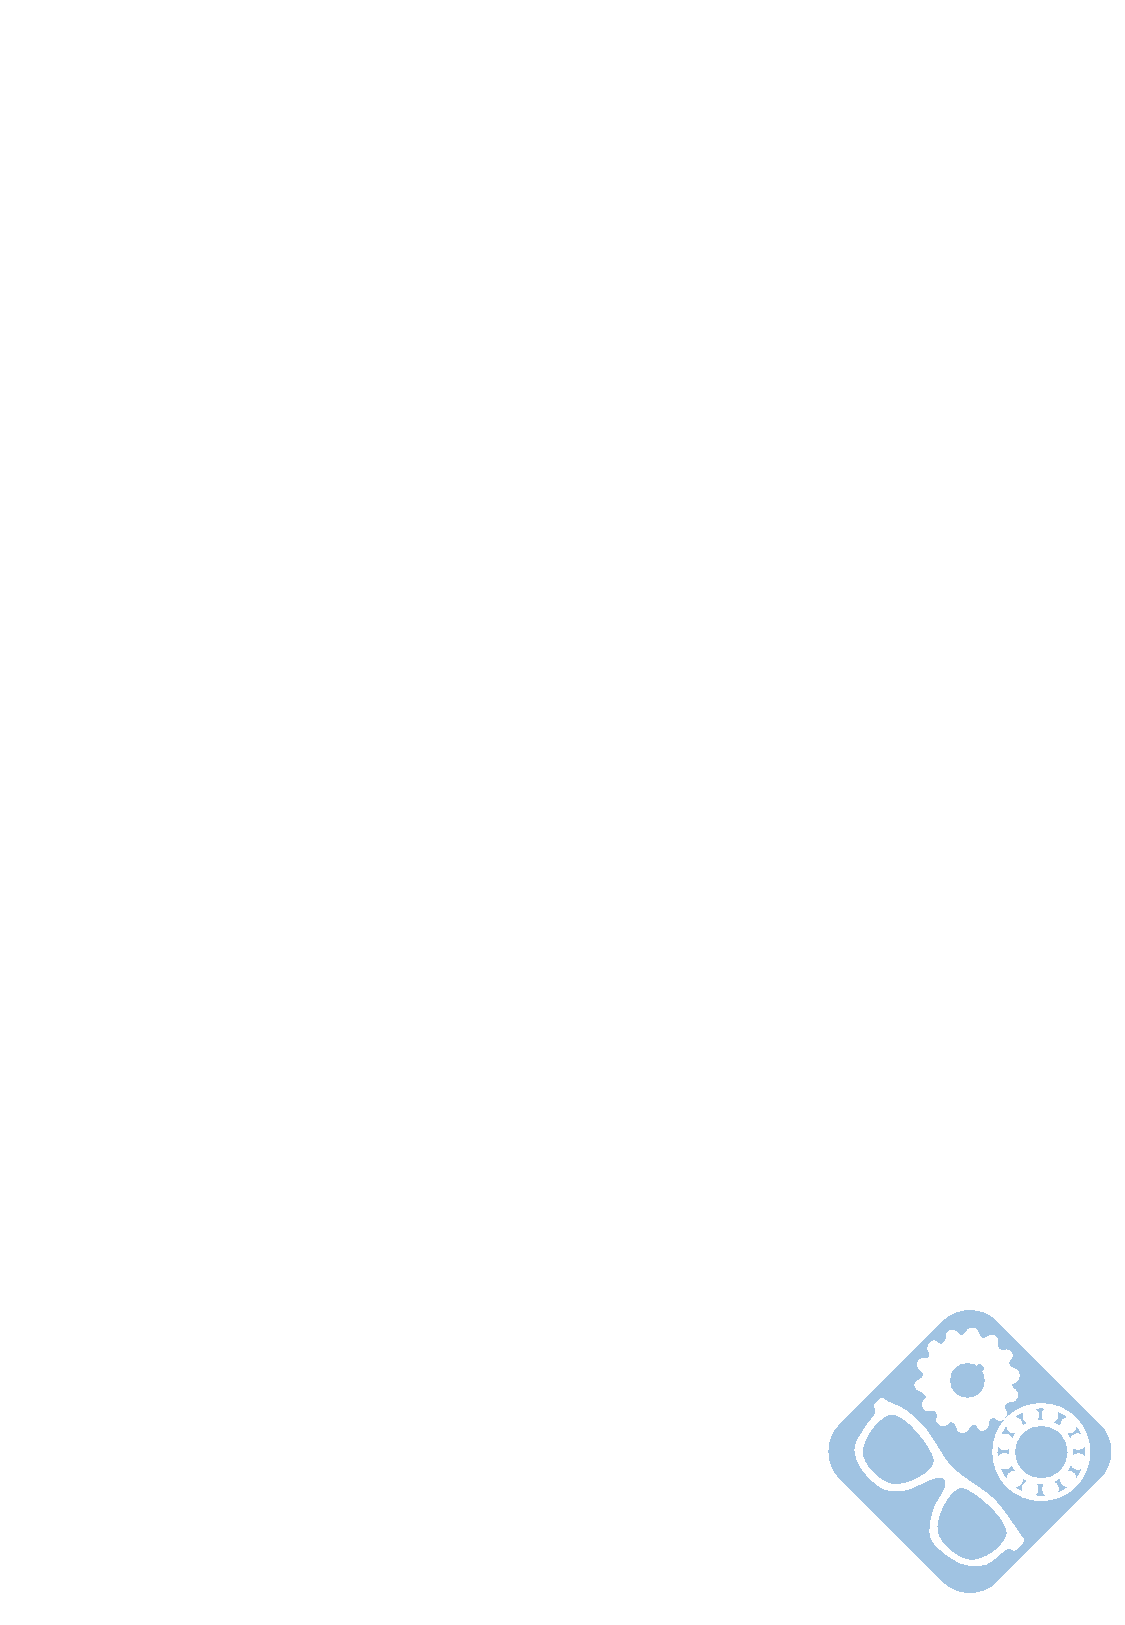
\includegraphics[width=\paperwidth,height=\paperheight,%
keepaspectratio]{../../../img/fond4}%
\end{center}
\vfill
}}}

\begin{document}

\pagestyle{empty}

\AddToShipoutPicture*{\BackgroundPic}


\includegraphics[width=2cm]{../../../img/logo}

\Huge{DS \numero - \sujet}

\vspace{1cm}

\ifdef{\prive}{\begin{center}\colorbox{danger}{\Huge{Avec Correction}}\end{center}}{}

\begin{center}
\centering\huge{PTSI}
\end{center}

\vspace{2cm}


\begin{center}
\centering\Large{\jour}
\end{center}

\vspace{2cm}

\normalsize

\tableofcontents

\newpage

\AddToShipoutPicture{\BackgroundPicdeux}

\pagestyle{fancy}

\begin{center}
\Huge \sujet
\end{center}


\normalsize


\paragraph{Contexte} ~\

L'autofocus (AF) est le terme anglais pour désigner la mise au point automatique. C'est une fonction qui permet la mise au point automatique de certains systèmes optiques comme les appareils photo, leur permettant
de régler la netteté du sujet. Cette mise au point est réalisée grâce à l'association d'un boîtier et d'un objectif photographiques.

\begin{figure}[!h]
\centering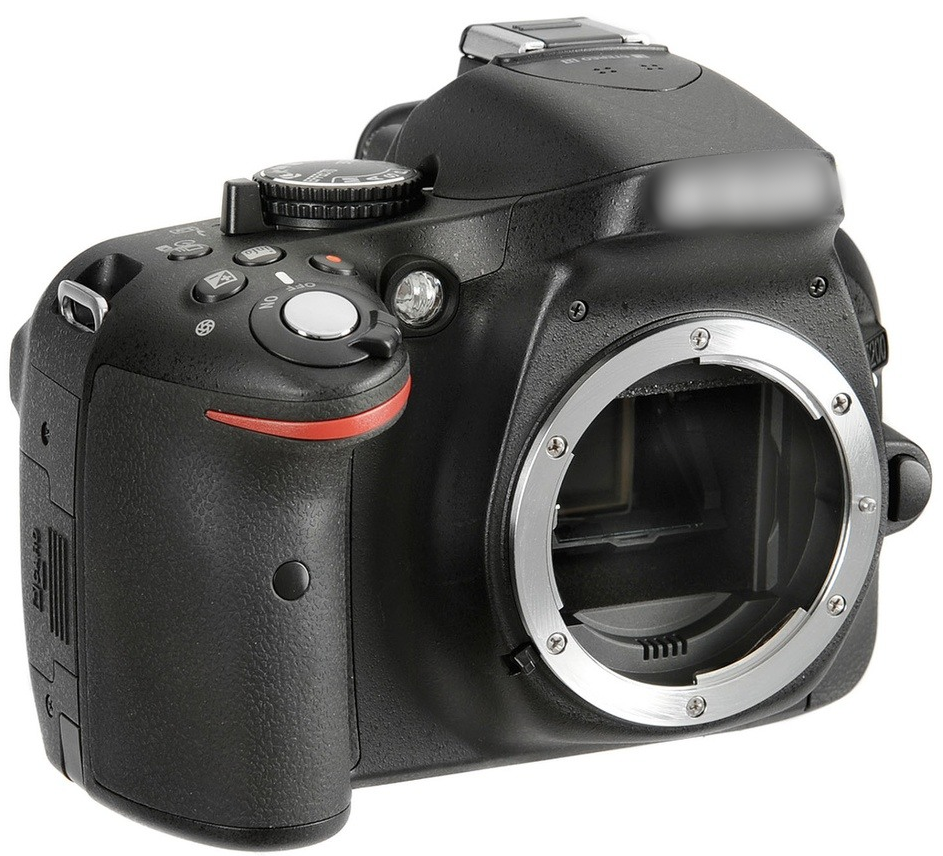
\includegraphics[width=0.3\linewidth]{img/figure_01_1}
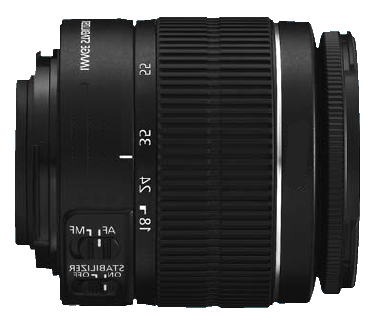
\includegraphics[width=0.3\linewidth]{img/figure_01_2}
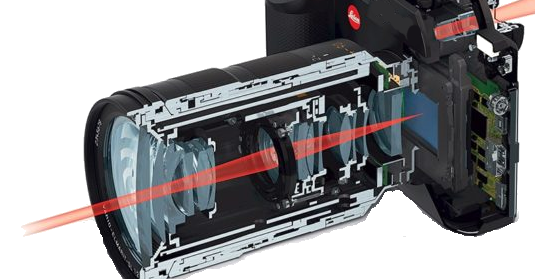
\includegraphics[width=0.3\linewidth]{img/figure_01_3}
 \caption{Boîtier et objectif photographiques}
 \label{img01}
\end{figure}

Le principe consiste à déplacer une lentille afin que les rayons de l'image à photographier convergent sur le capteur. Si ce n'est pas le cas, l'image sera floue. Sur la figure \ref{img02}, la lentille est bien positionnée uniquement sur le schéma du milieu : les rayons convergent parfaitement sur le capteur.

\begin{figure}[!h]
\centering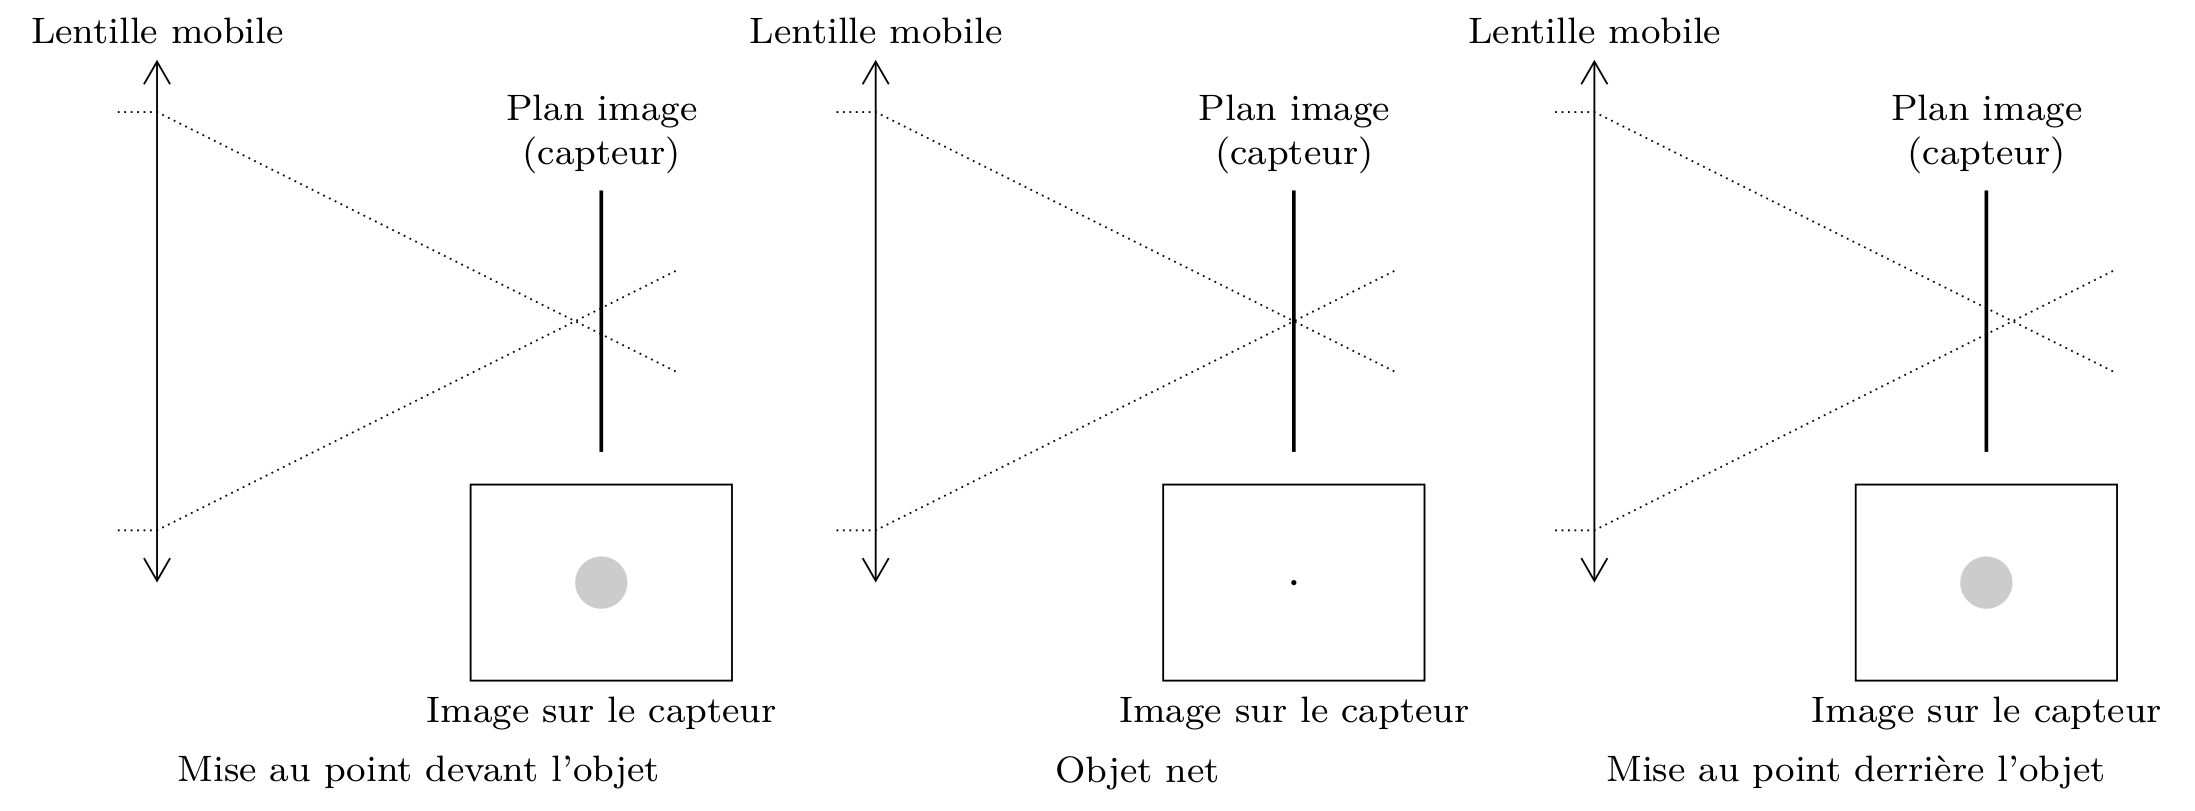
\includegraphics[width=0.9\linewidth]{img/figure_02}
 \caption{Principe de la mise au point (source : http://www.pierretoscani.com/autofocus.html)}
 \label{img02}
\end{figure}

La qualité de la mise au point dépend de plusieurs facteurs techniques et logiciels. Dans ce sujet, seules les exigences relatives au déplacement de la lentille mobile seront étudiées.

\paragraph{Mise en situation} ~\

Le mouvement de la lentille est donné par l'architecture représentée figure \ref{img03}.

L'architecture détaillée est donnée en figure \ref{img04}. La modélisation acausale correspondante de l'objectif photographique est donnée figure \ref{img05}.

\newpage

\begin{figure}[!h]
\centering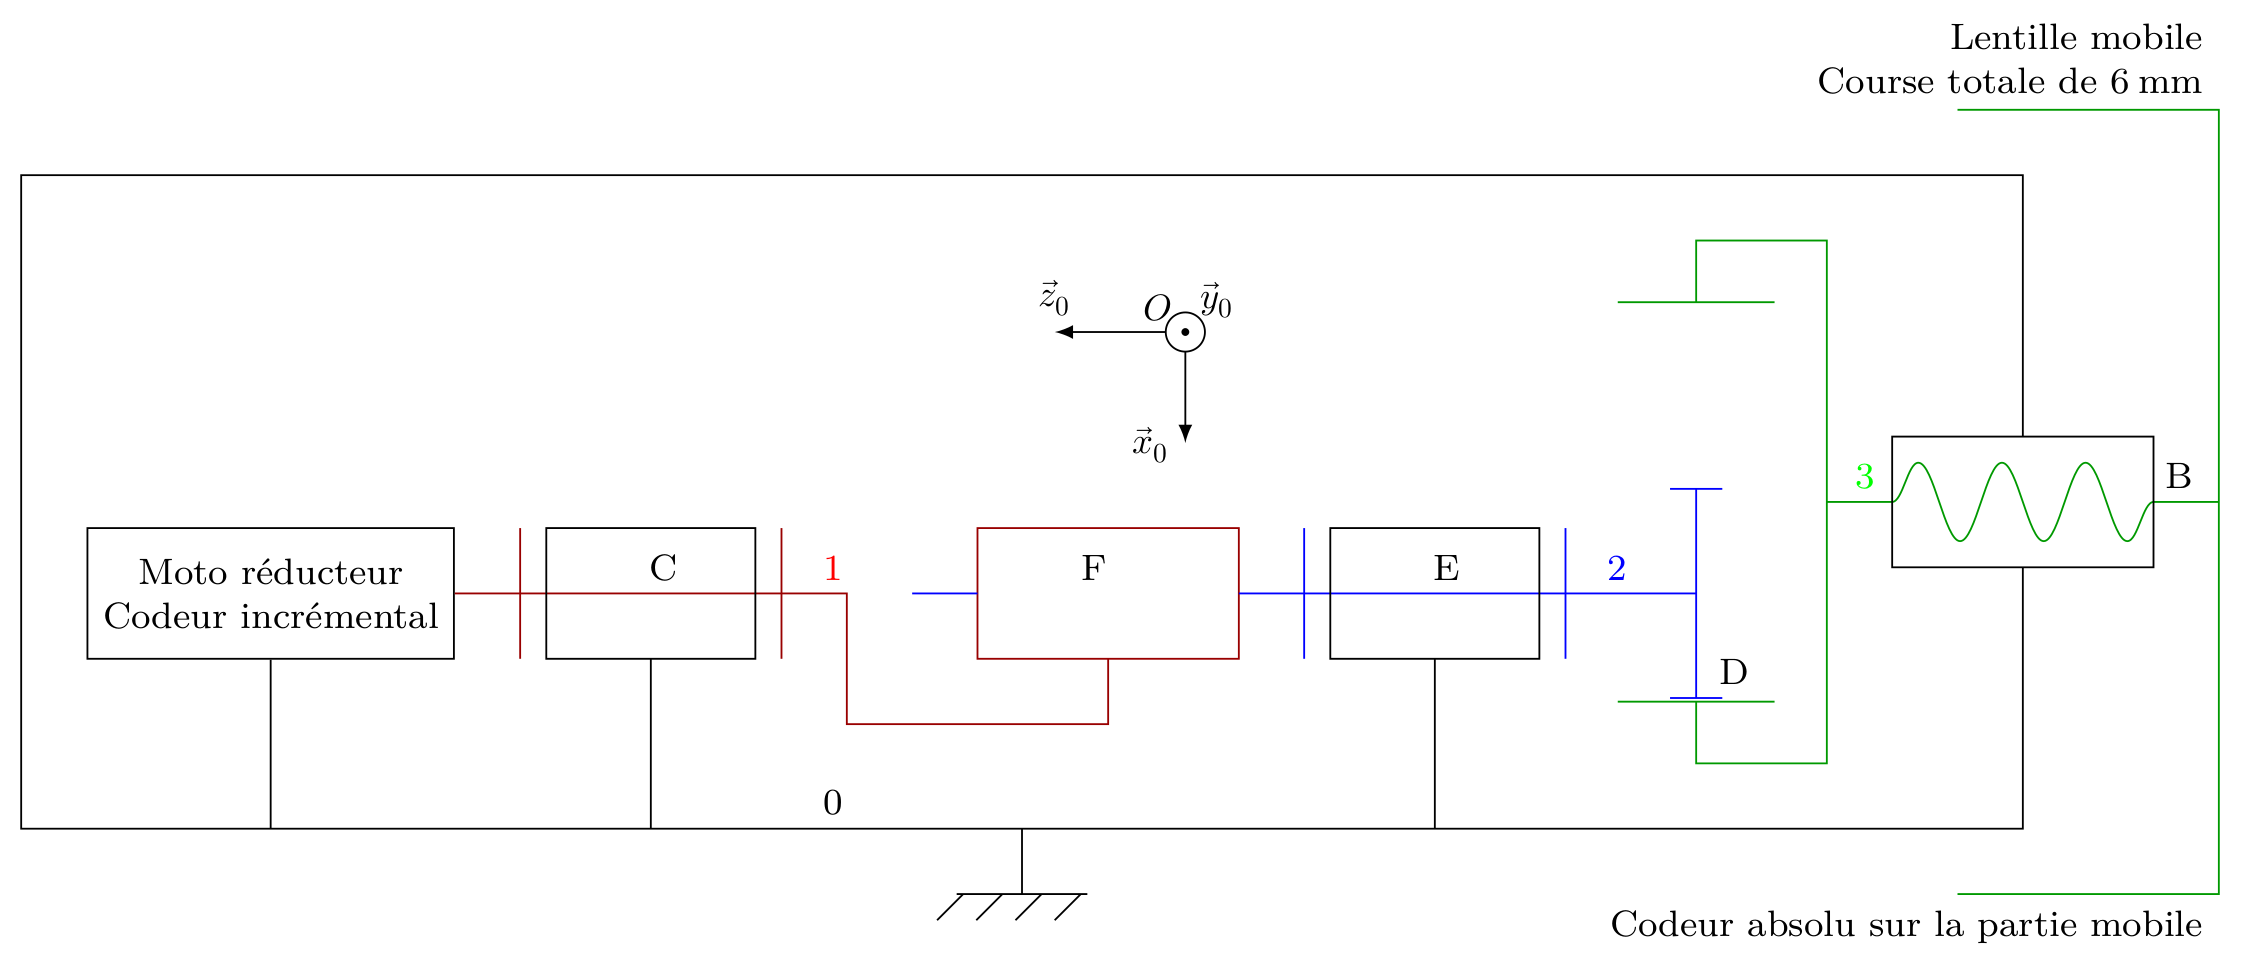
\includegraphics[width=0.82\linewidth]{img/figure_03}
 \caption{Architecture du dispositif de déplacement de la lentille}
 \label{img03}
\end{figure}

\begin{figure}[!h]
\centering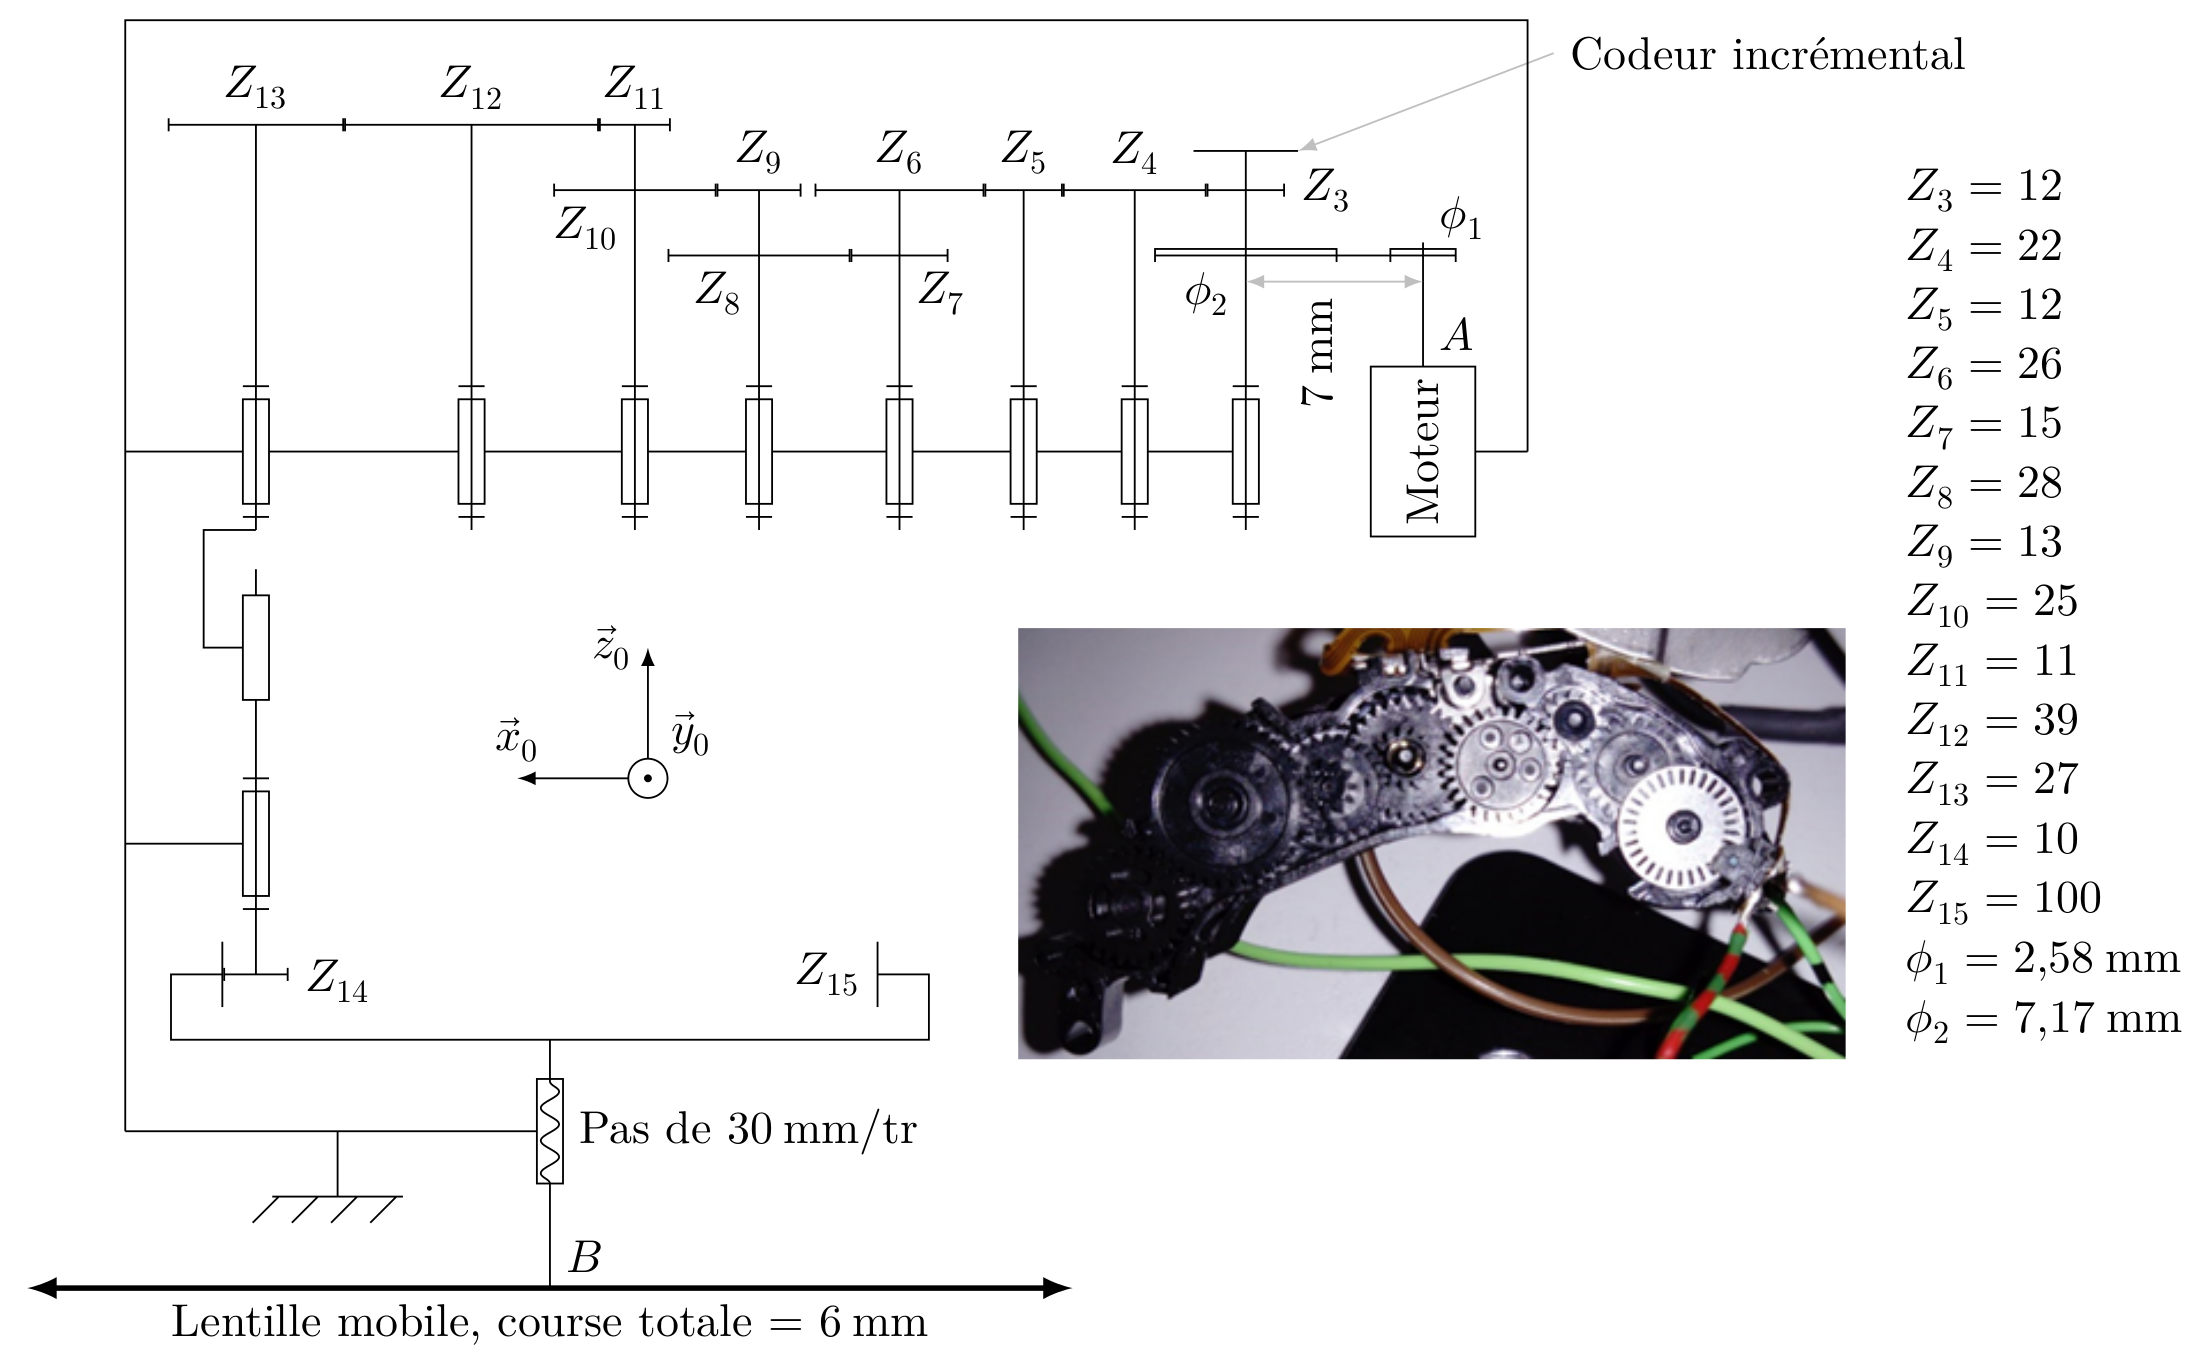
\includegraphics[width=0.85\linewidth]{img/figure_04}
 \caption{Schéma cinématique du mécanisme de déplacement de la lentille}
 \label{img04}
\end{figure}

\begin{figure}[!h]
\centering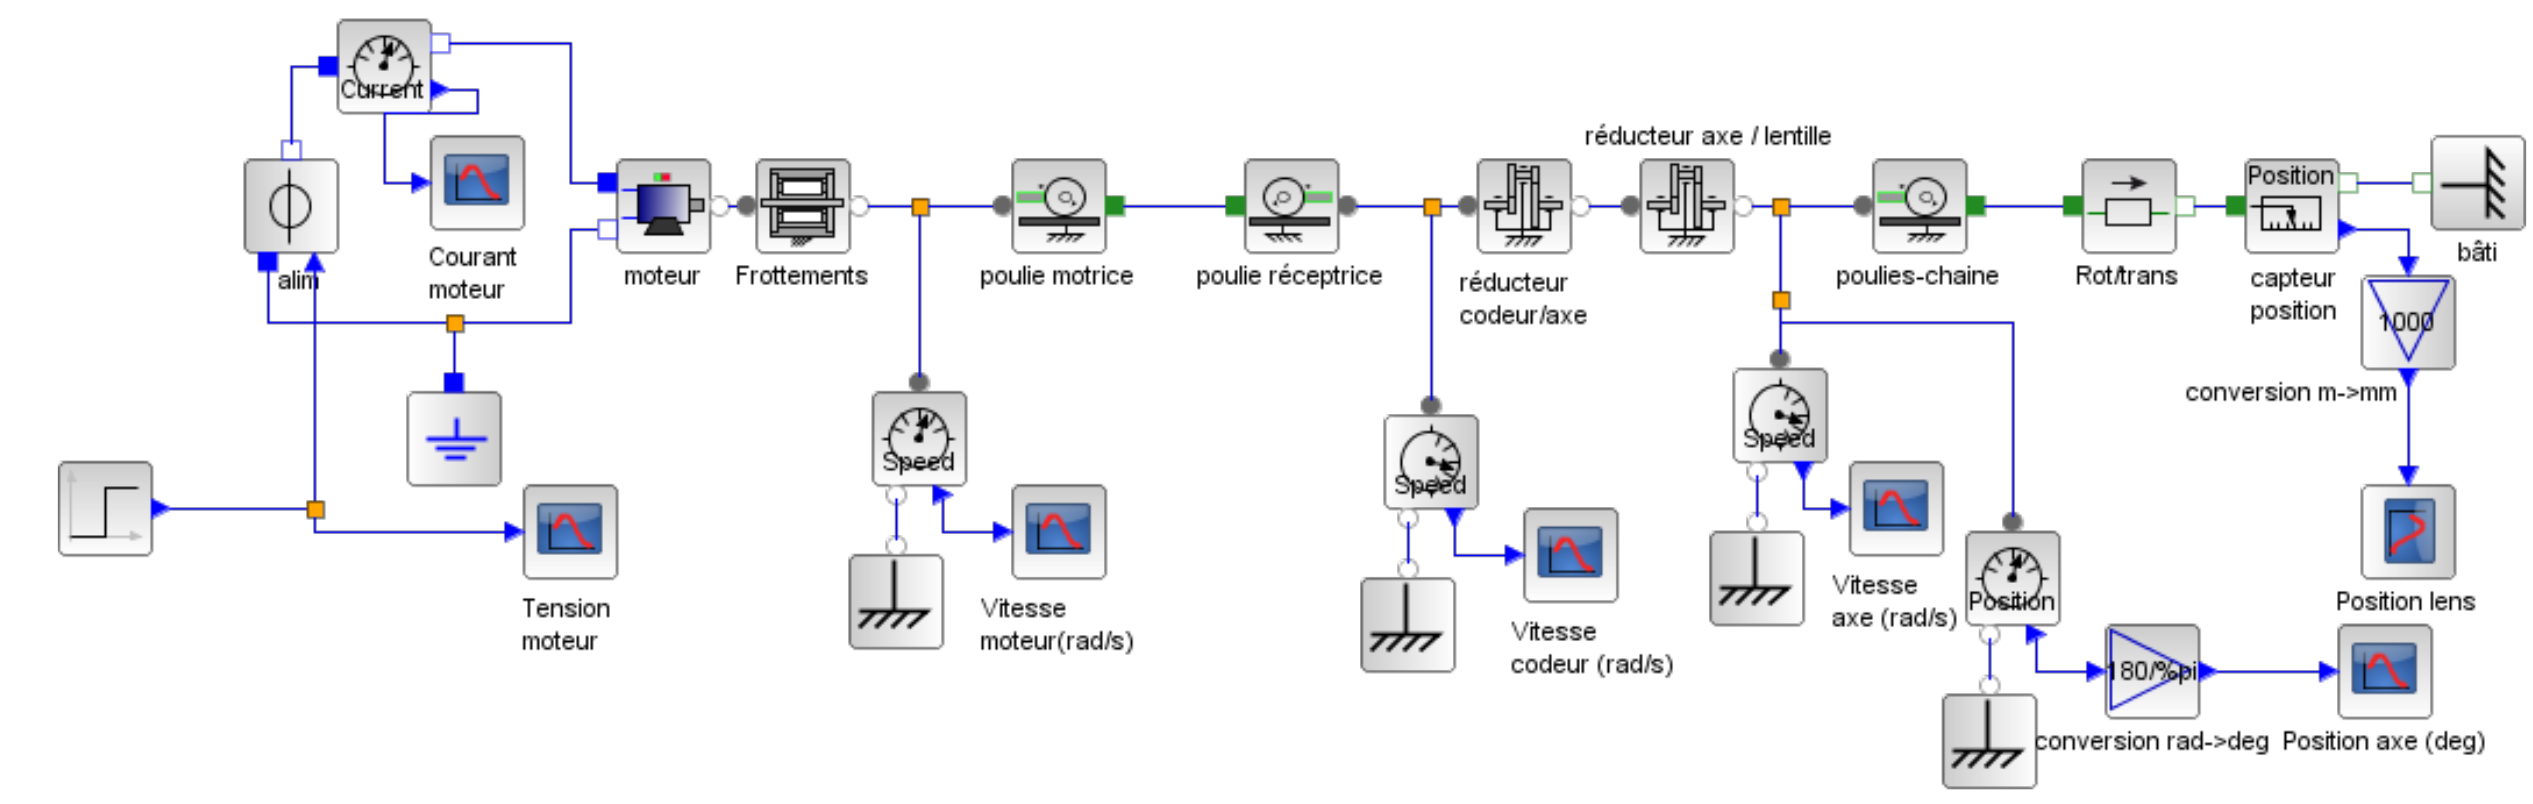
\includegraphics[width=0.9\linewidth]{img/figure_05}
 \caption{Architecture du dispositif de déplacement de la lentille}
 \label{img05}
\end{figure}

\newpage

\paragraph{Extrait du cahier des charges} ~\

\begin{figure}[!h]
\centering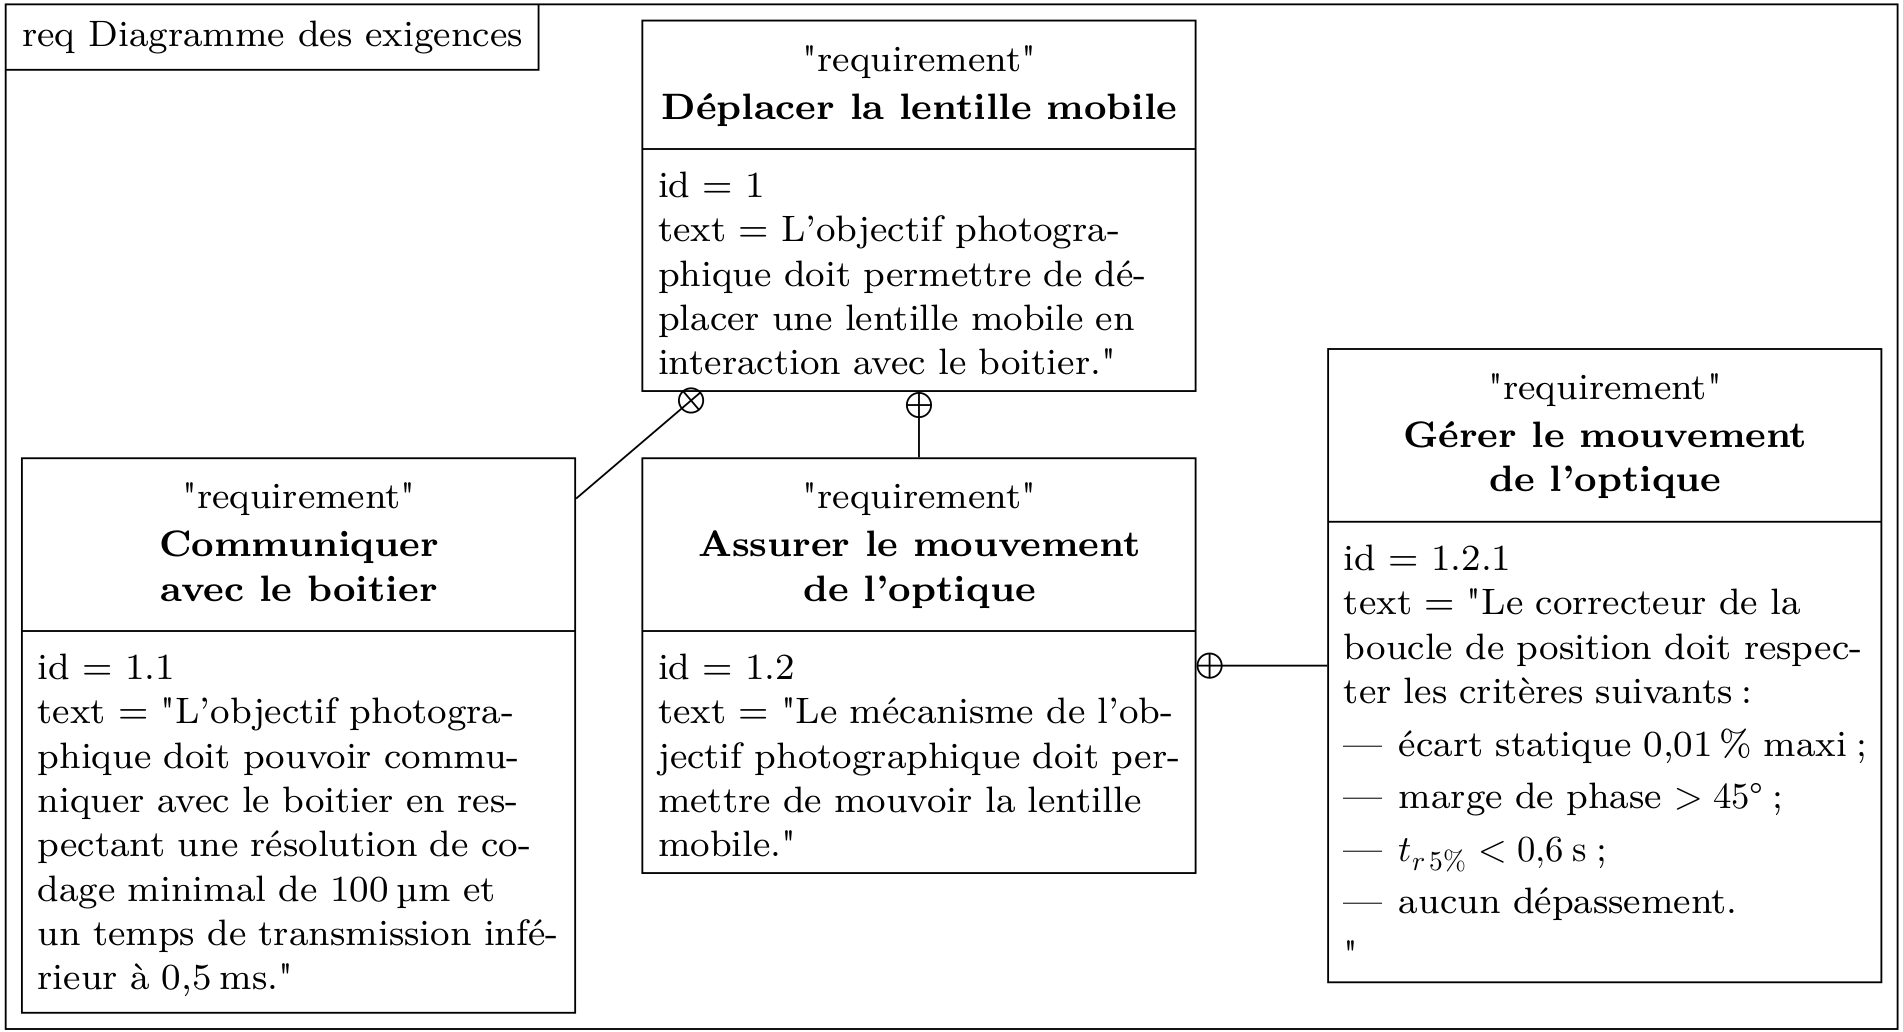
\includegraphics[width=0.9\linewidth]{img/figure_06}
 \caption{Exigences extraites du cahier des charges}
 \label{img06}
\end{figure}

\paragraph{Objectif final} ~\

Le sujet a pour but de modéliser, analyser et améliorer les performances de l'objectif photographique. Pour cela, il comporte trois parties avec comme buts :
\begin{itemize}
 \item valider la communication entre le boitier et l'objectif photographique permettant la mise au point et déterminer la consigne qui doit être envoyée par le boitier : il est question de valider le temps de communication qui doit être négligeable devant la dynamique du système,
 \item modéliser la structure permettant d'\og assurer le mouvement de l'optique \fg : cette partie permet de modéliser et de déterminer numériquement les frottements au travers de mesures, ces grandeurs sont fondamentales car les non linéarités vont fortement influencer la commande,
 \item choisir et régler le correcteur permettant de \og gérer le mouvement de l'optique \fg : cette partie permet de trouver le bon compromis de réglage de la commande afin de respecter les critères du cahier des charges.
\end{itemize}

\section{Communication entre le boitier et l'objectif photographique}

\paragraph{Objectif} ~\

Valider le protocole de communication utilisé entre le boitier et l'objectif photographique en termes de débit de transmission et de résolution de codage afin qu'il réponde aux exigences de la mise au point. Déterminer la consigne qui doit être envoyée en entrée de l'asservissement en position de la lentille.

La mise au point résulte de l'interaction entre le boitier où se situe tout le traitement de numérisation de l'image (capteur CCD et programme de mise au point) et l'objectif photographique qui permet de mouvoir la
lentille. Afin de réaliser correctement cette mise au point, il est nécessaire que l'objectif photographique puisse communiquer avec tous les boitiers compatibles en répondant aux exigences suivantes.

\begin{center}
\begin{tabular}{|p{6.7cm}|p{7cm}|p{1.7cm}|}
\hline
Exigence & Critère d'appréciation & Niveau \\
\hline
\multirow{2}{*}{Id = « 1.1 » Communiquer avec le boitier} & Temps de transmission d'un échange entre l'objectif
photographique et le boitier & $<0.5ms$\\
\cline{2-3}
& Résolution de codage & $< 100 \mu m$\\
\hline
\end{tabular}
\end{center}

Lorsque l'utilisateur appuie sur le déclencheur, l'objectif photographique entre dans une phase d'initialisation durant laquelle la lentille mobile (figure 4) se déplace de la mise au point minimale à la mise au point infinie, ce qui correspond à sa course totale.

L'objectif photographique est équipé de deux capteurs permettant de mesurer le déplacement de la lentille :
\begin{itemize}
 \item un codeur absolu linéaire 4 bits, situé au niveau de la lentille mobile, permettant de connaître la position de la lentille mobile selon la direction $\vec{z}_0$ de la figure \ref{img04},
\begin{center}
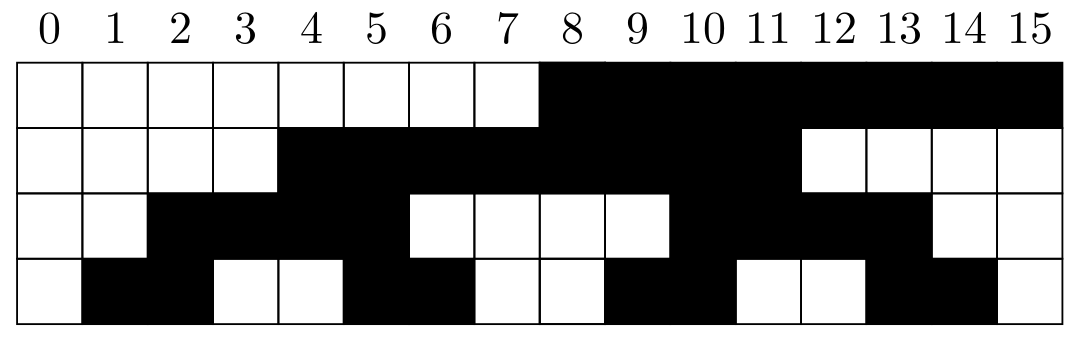
\includegraphics[width=0.6\linewidth]{img/image_01}
\end{center} 
 \item un codeur incrémental (monovoie, 30 impulsions par tour) relié à la MCC (Machine à Courant Continu) par un dispositif poulies-courroie (figure \ref{img04}).
 \begin{center}
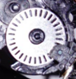
\includegraphics[width=0.2\linewidth]{img/image_02}
\end{center} 
\end{itemize}

Pour obtenir une zone de mise au point la plus nette possible, il est nécessaire que la résolution au niveau du positionnement de la lentille mobile soit inférieure à $100 \mu m$.

\question{Donner la résolution possible pour la course totale de la lentille mobile avec le codeur absolu. Justifier
que le codeur absolu ne soit utilisé que lors de la phase d'initialisation de l'objectif photographique.}

\question{Déterminer la relation entre le déplacement de la lentille mobile $d_l$ et la position angulaire du codeur incrémental $\theta_{rc}$ . En déduire la résolution possible pour la course totale de la lentille, si elle est déterminée en comptant les impulsions du codeur incrémental sur les fronts montants.}

~\

Dans la suite, la résolution sera prise égale à $5 \mu m$.

\question{En déduire le nombre de bits nécessaires pour coder l'information \og déplacement de la lentille mobile \fg,
si cette dernière est donnée par le comptage du nombre d'impulsions au niveau du codeur incrémental.}

~\

Les objectifs photographiques de la marque Canon sont reliés aux boitiers via sept connexions permettant la communication entre ces deux parties. Le protocole de communication utilisé entre le boitier et l'objectif photographique est de type maitre-esclave et utilise la communication série SPI. Le détail est donné figure \ref{img07}.

\begin{figure}[!h]
\centering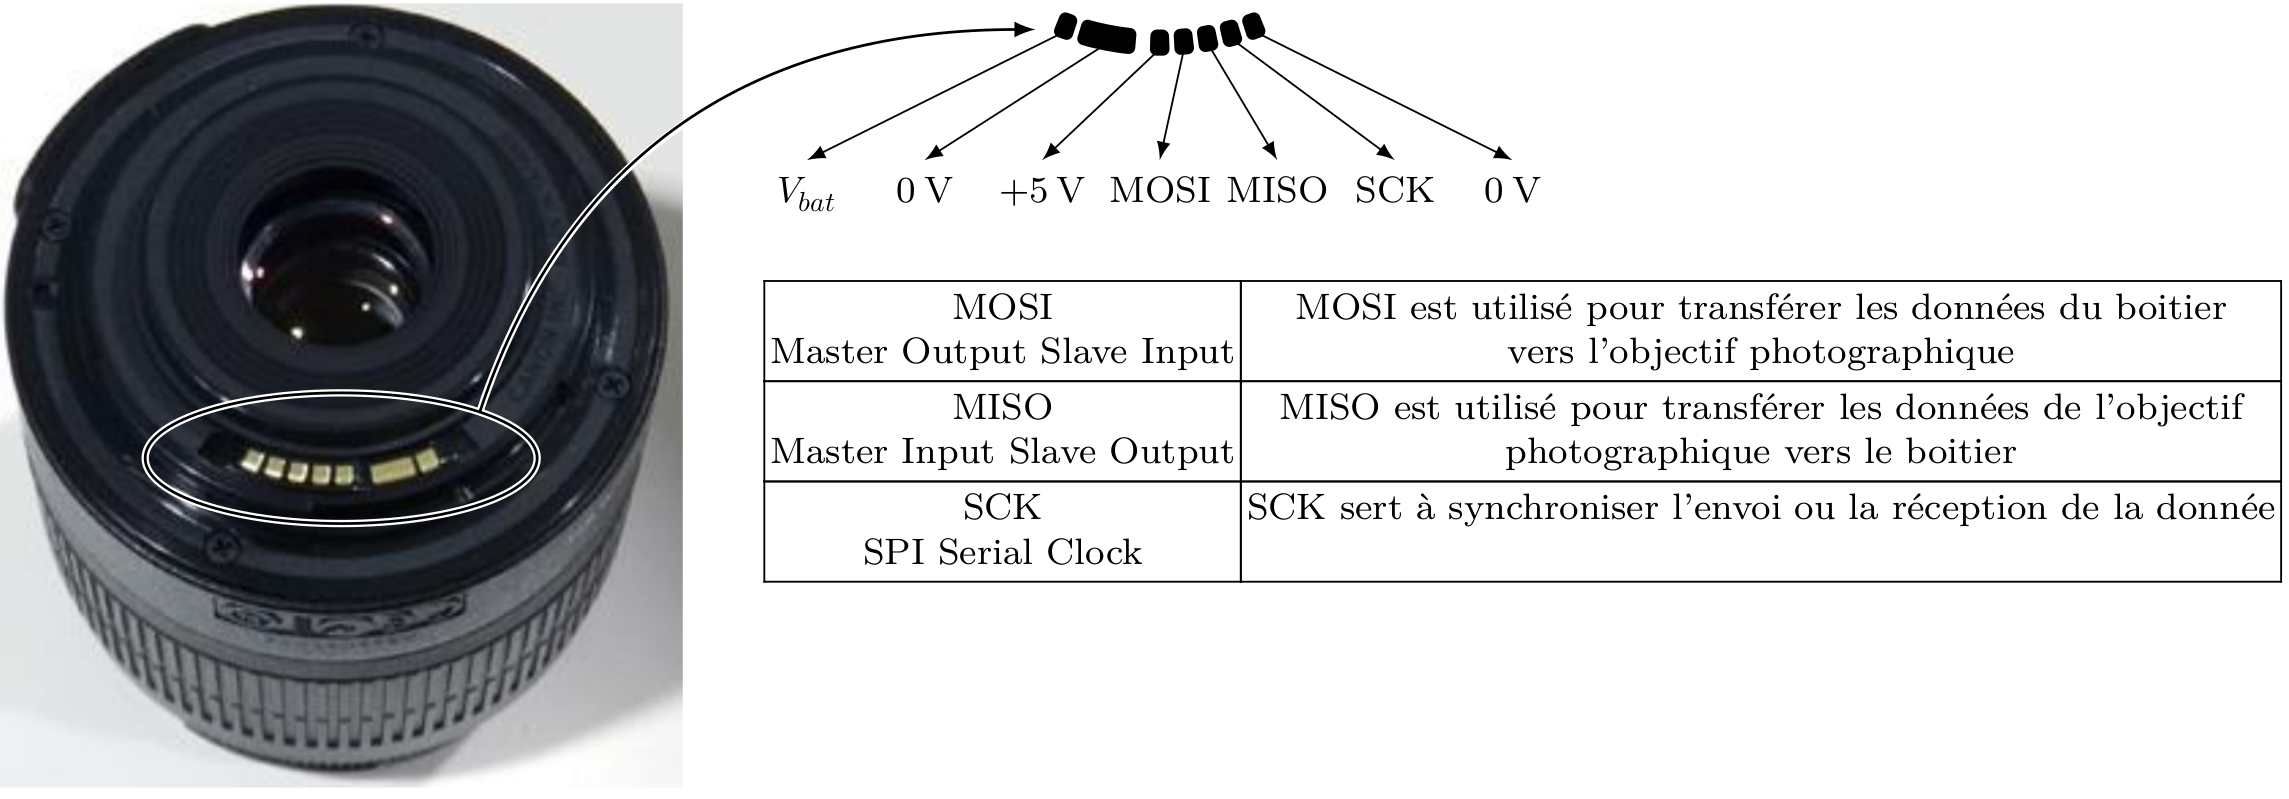
\includegraphics[width=0.9\linewidth]{img/figure_07}
 \caption{Communication SPI entre le boitier et l'objectif photographique}
  \label{img07}
\end{figure}

Les valeurs sur $MISO$ et $MOSI$ sont lues et interprétées sur les fronts montants (passage de $0$ à $1$) du signal d'horloge $SCK$. Un $0$ logique est codé par une tension de $0V$ et un $1$ logique est codé par une tension de $5V$. La transmission se fait octet par octet, le bit de poids fort en premier.

Lors d'un essai de mise au point, une trame de communication entre le boitier et l'objectif photographique a été interceptée. Cette trame, représentée figure A du document réponse, contient la valeur de l'ordre de déplacement demandée par le boitier à l'objectif photographique, codée sur deux octets. L'octet de poids fort est transmis en premier.

\question{Indiquer le contenu des deux octets transmis par le boitier sur le tableau du document réponse.}

\question{Décoder l'ordre de déplacement de la lentille mobile, codé sur un entier signé 16 bits, envoyé à l'objectif photographique. En déduire le déplacement en mm qui a été demandé lors de l'essai qui sera réalisé en dernière partie pour le réglage du correcteur.}

~\

Lors de la demande de déplacement de la lentille mobile, le boitier va transmettre à l'objectif photographique une trame de trois octets, via la ligne MOSI : une commande sur un octet puis, l'ordre de déplacement codé sur deux octets. L'objectif photographique confirme la prise en compte de ces informations en full-duplex via la ligne MISO.

Afin que la communication entre le boitier et l'objectif photographique n'ait pas d'impact sur la dynamique du système, il est nécessaire qu'un échange pour la consigne de déplacement entre le boitier et l'objectif photographique soit réalisé en moins de $0.5ms$.

\question{Donner, à partir de la figure A du document réponse et de l'explication précédente, le temps de transmission $t_{com}$ nécessaire pour un échange entre le boitier et l'objectif photographique. Conclure vis-à-vis de l'exigence Id 1.1.}

\section{Validation de la structure permettant d'assurer le mouvement
de l'optique}

\paragraph{Objectif}

Valider la structure qui permet de faire translater la lentille mobile et de déterminer les différents paramètres du modèle multi-physique de l'objectif photographique.

Afin de vérifier et d'améliorer les performances de l'objectif photographique, il est nécessaire de déterminer les différents paramètres du modèle multi-physique donné précédemment. La démarche adoptée ici est la suivante :
\begin{itemize}
 \item détermination de l'équation de mouvement au niveau de la MCC,
 \item détermination des paramètres du modèle de la MCC,
 \item modélisation du frottement sec et du frottement visqueux.
\end{itemize}

\subsection{Détermination du mouvement}

\paragraph{Objectif}

Déterminer l'équation de mouvement qui sera utilisée dans le modèle de la commande.

Le dispositif permettant de mouvoir la lentille mobile ainsi que toutes ses caractéristiques sont données en figure \ref{img04}.

\paragraph{Hypothèses et notations} ~\

Les hypothèses sont :
\begin{itemize}
 \item la courroie ne glisse pas ;
 \item l'action de la pesanteur est négligée.
\end{itemize}

Les seules masses et inertie à prendre en compte sont :
\begin{itemize}
 \item la masse de la lentille notée $M$,
 \item l'inertie équivalente des éléments mobiles $J$.
\end{itemize}

Les mouvements sont :
\begin{itemize}
 \item $\left\{V_{mot/0}\right\}_A=\left\{\begin{array}{c}
 \omega_m\cdot\vec{z}_0 \\
 \vec{0} 
 \end{array}\right\}_A$,
 \item $\left\{V_{lentille/0}\right\}_B=\left\{\begin{array}{c}
 \omega_l\cdot\vec{z}_0 \\
 V_l\cdot\vec{z}_0
 \end{array}\right\}_B$
\end{itemize}

\question{Calculer la valeur numérique du rapport de réduction du réducteur $k=\frac{\omega_l}{\omega_m}$.}

~\

L'ensemble isolé est constitué de toutes les pièces mobiles de la figure 4.

En utilisant le théorème de l'énergie cinétique, l'équation de mouvement s'écrit :
\begin{center}
$C_m-C_0=J\cdot\dfrac{d\omega_m}{dt}+f\cdot\omega_m$.
\end{center}

\subsection{Étude des contraintes sur le positionnement}

\paragraph{Objectif}

Étudier l'hyperstatisme du mécanisme de déplacement de la lentille dans le but qu'il soit isostatique pour limiter l'impact des frottements.

La modèle du mécanisme de déplacement de la lentille mobile est donné sur la figure \ref{img08}

\begin{figure}[!h]
\centering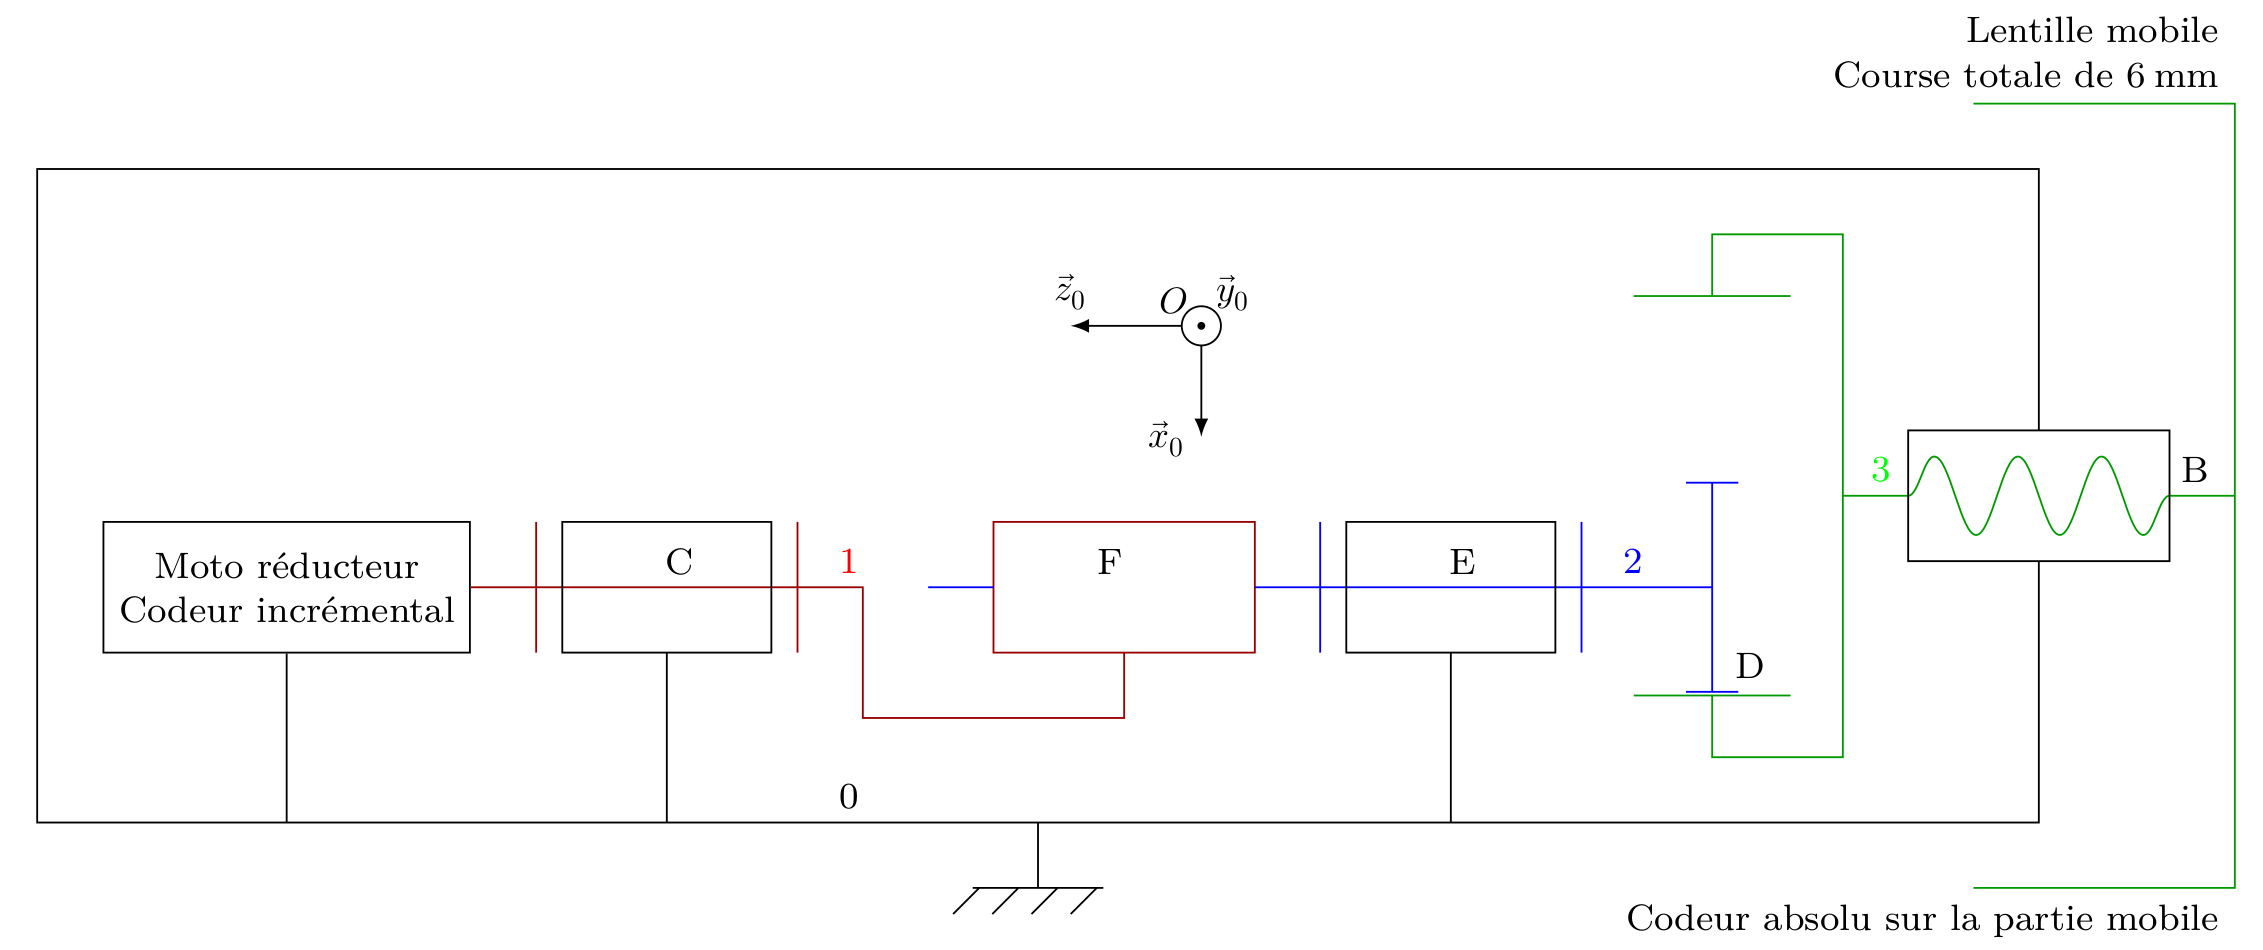
\includegraphics[width=0.9\linewidth]{img/figure_08}
 \caption{Exigences extraites du cahier des charges}
 \label{img08}
\end{figure}

On notera les distances $\overrightarrow{DB}=a\cdot\vec{x}_0+b\cdot\vec{z}_0$ et $\overrightarrow{DE}=c\cdot\vec{x}_0+d\cdot\vec{z}_0$. On remarquera que $C$, $F$ et $E$ sont alignés selon $\vec{z}_0$. Les torseurs cinématiques des différentes liaisons
sont :

$\left\{V_{1/0}\right\}=\left\{\begin{array}{c}
 \omega_{1/0}\cdot\vec{z}_0 \\
 \vec{0} 
 \end{array}\right\}_C$,
$\left\{V_{3/0}\right\}=\left\{\begin{array}{c}
 \omega_{3/0}\cdot\vec{z}_0 \\
 p\cdot\omega_{3/0}\cdot\vec{z}_0 \\
 \end{array}\right\}_B$,
 $\left\{V_{2/0}\right\}=\left\{\begin{array}{c}
 \omega_{2/0}\cdot\vec{z}_0 \\
 \vec{0} 
 \end{array}\right\}_E$,

 $\left\{V_{3/2}\right\}=\left\{\begin{array}{cc}
 \omega_{3/2x} & V_{3/2x} \\
 \omega_{3/2y} & 0 \\
 \omega_{3/2z} & V_{3/2z} 
 \end{array}\right\}_{D,R_0}$,
 $\left\{V_{2/1}\right\}=\left\{\begin{array}{c}
 \vec{0} \\
 V_{2/1}\cdot\vec{z}_0 
 \end{array}\right\}_C$,

\question{Écrire les fermetures cinématiques des chaines 0-1-2 au point C et 0-2-3 au point D.}

\question{Écrire les douze équations associées aux fermetures précédentes et les mettre sous la forme de matrice donnée ci-dessous, en remplaçant les points d'interrogation.}

\begin{center}
$\left(\begin{array}{ccccccccc}
0&0&0&0&0&0&0&0&0\\
0&0&0&0&0&0&0&0&0\\
?&0&?&0&0&0&0&0&0\\
0&0&0&0&0&0&0&0&0\\
0&0&0&0&0&0&0&0&0\\
0&?&0&0&0&0&0&0&0\\
0&0&0&0&?&0&0&0&0\\
0&0&0&0&0&?&0&0&0\\
0&0&?&?&0&0&?&0&0\\
0&0&0&0&0&0&0&?&0\\
0&0&?&?&0&0&0&0&0\\
0&0&0&?&0&0&0&0&?\\
\end{array}\right)\cdot
\left(\begin{array}{c}
\omega_{1/0} \\
V_{2/1} \\
\omega_{2/0} \\
\omega_{3/0} \\
\omega_{3/2x} \\
\omega_{3/2y} \\
\omega_{3/2z} \\
V_{3/2x} \\
V_{3/2z}
\end{array}\right)=
\left(\begin{array}{c}
0\\0\\0\\0\\0\\0\\0\\0\\0\\0\\0\\0	
\end{array}\right)
$
\end{center}

\question{Sans calculs, mais avec justification, donner le rang de la matrice. En déduire, la mobilité m du modèle du mécanisme.}

\question{Calculer le degré d'hyperstatisme du modèle du mécanisme.}

L'analyse des lignes de zéros de la matrice permet de déterminer les contraintes géométriques et d'orientation du mécanisme liées à l'hyperstatisme.

\question{Proposer un nouveau modèle pour les deux liaisons pivots afin de rendre le modèle du mécanisme isostatique.}

\subsection{Détermination du modèle de la machine à courant continu}

\paragraph{Objectif}

Déterminer les paramètres du modèle de la MCC à partir de différents essais effectués sur le système
réel.

Afin d'identifier le modèle de la machine à courant continu, différents essais à rotor bloqué et en charge à différentes vitesses sont effectués. Ainsi, il est possible de déterminer expérimentalement les paramètres du modèle multiphysique suivants :
\begin{itemize}
 \item la résistance d'induit notée $R_m$,
 \item l'inductance d'induit, notée $L_m$,
 \item la constante de la force électromotrice, notée $K_e$,
 \item la constante de couple, notée $K_T$,
 \item le couple total de frottement sec ramené sur l'axe de la MCC, noté $C_0$,
 \item le moment d'inertie équivalent ramené sur l'axe de la MCC, noté $J$,
 \item le coefficient de frottement visqueux, noté $f$.
\end{itemize}

\question{Donner le schéma équivalent de l'induit de la machine à courant continu ainsi que les équations liant les paramètres énumérés précédemment. La vitesse de rotation de la MCC sera notée $\omega_m$, la tension d'induit $u_m$ et le courant d'induit $i_m$.}

Lors de l'essai de la machine à courant continu à rotor bloqué et sous tension d'induit réduite de $1.6V$, le courant d'induit $i_m(t)$ est mesuré. Les résultats sont donnés sur la figure \ref{img09}.

\begin{figure}[!h]
\centering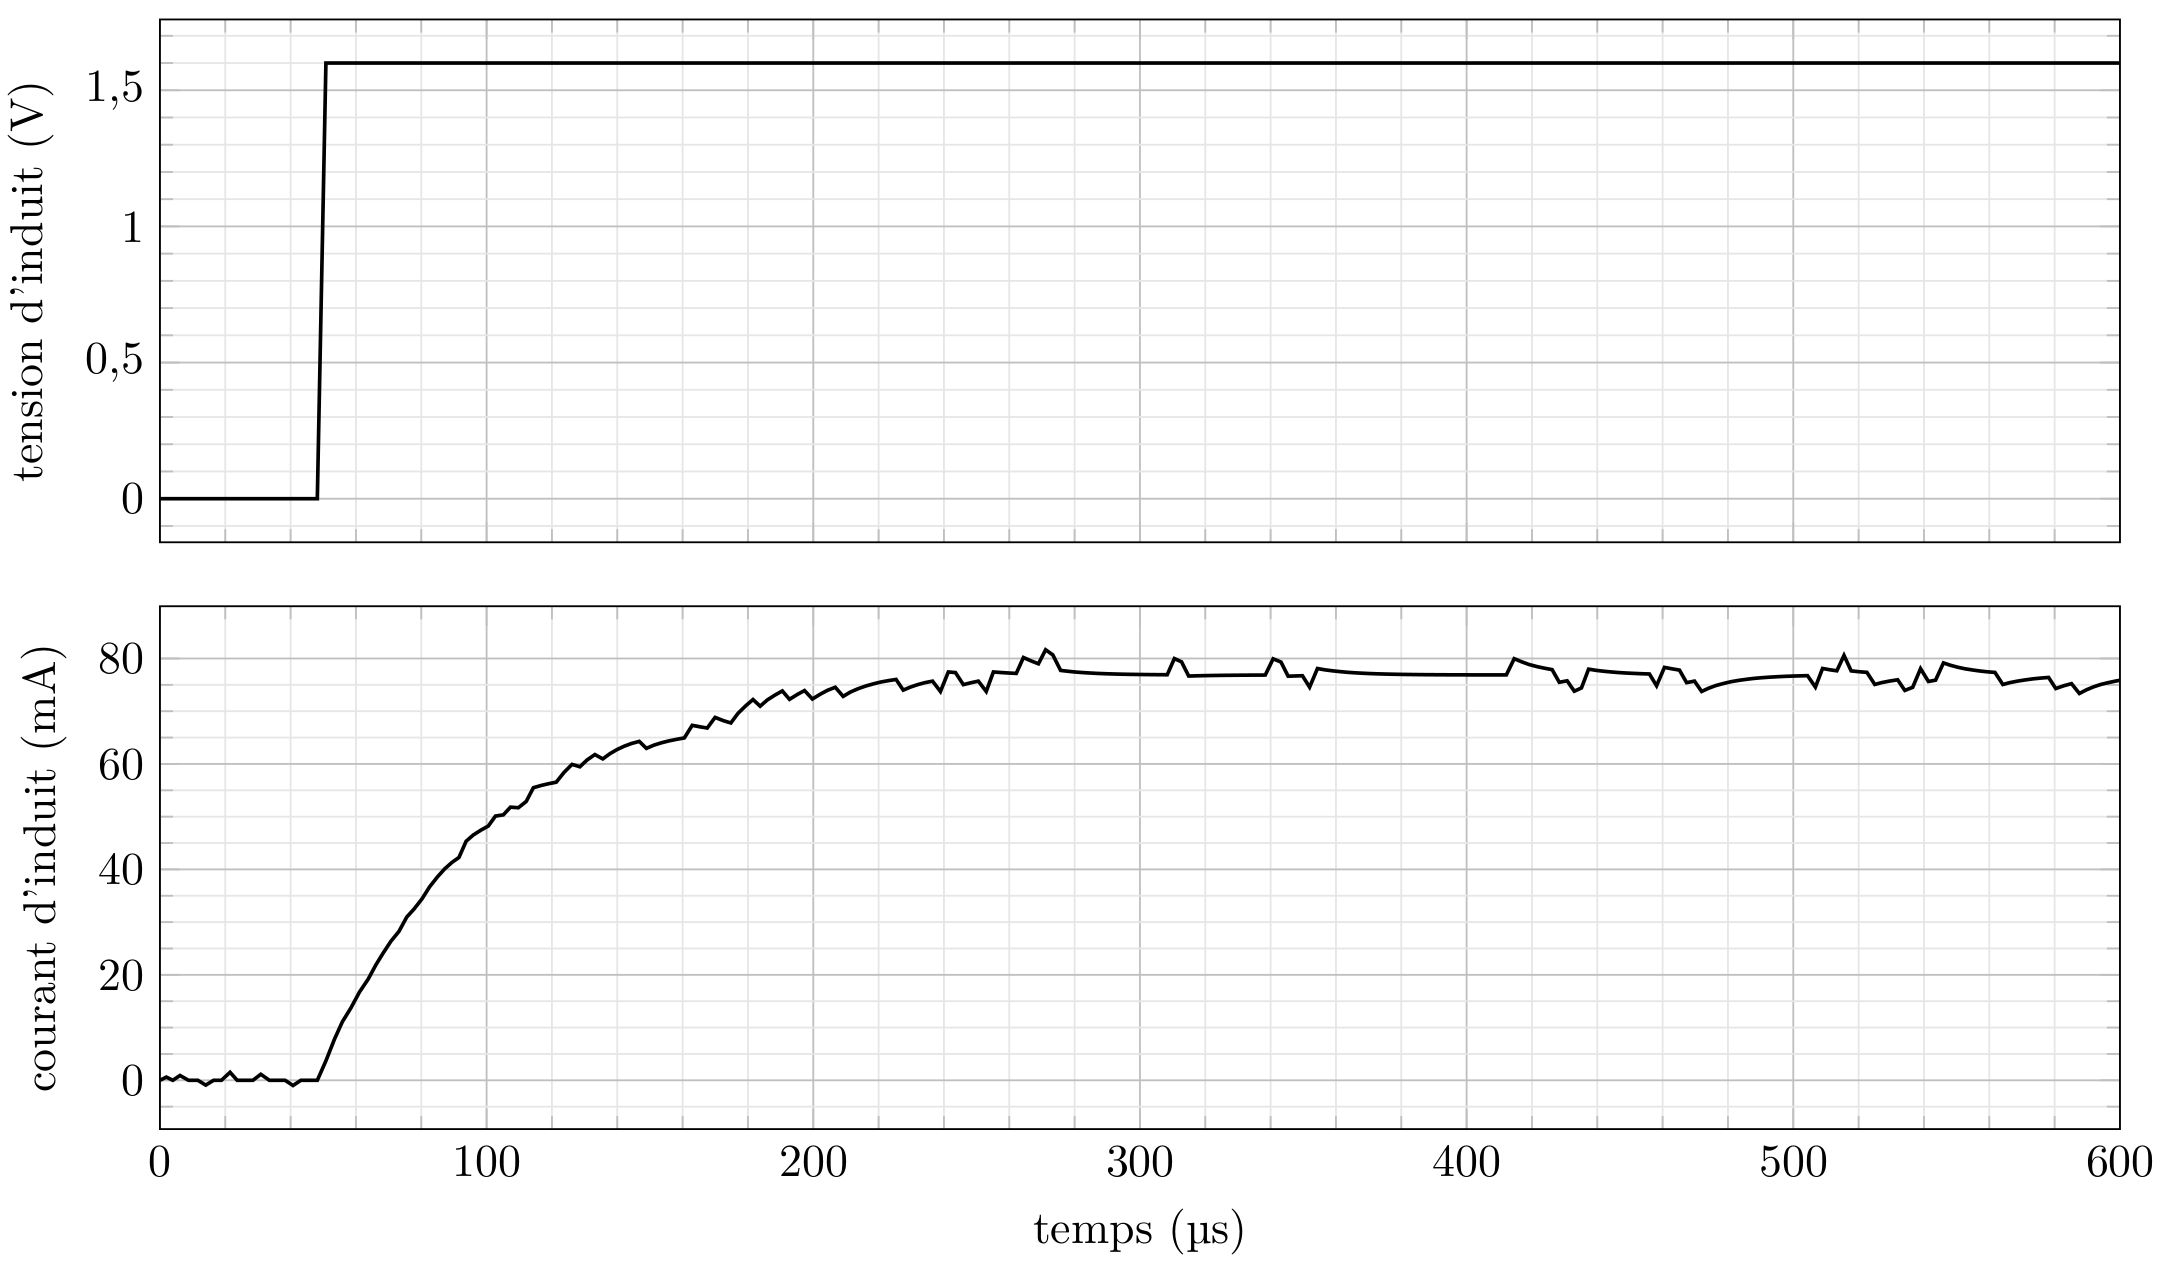
\includegraphics[width=0.8\linewidth]{img/figure_09}
 \caption{Résultats de l'essai de la MCC à rotor bloqué}
 \label{img09}
\end{figure}

\question{Déterminer la résistance d'induit $R_m$ et l'inductance d'induit $L_m$ à partir de l'essai à rotor bloqué et des équations précédentes.}

Afin de déterminer les autres paramètres de la machine à courant continu et de l'ensemble en mouvement, plusieurs essais pour différentes tensions d'induit sont réalisés. Le courant d'induit $i_m$ est mesuré à l'aide d'une pince ampèremétrique et les impulsions issues du codeur incrémental sont comptées et chronométrées à l'aide d'interruptions sur un microcontrôleur.

Afin de déterminer la constante de force électro-motrice $K_e$, il est nécessaire de déterminer une relation entre la tension d'induit $u_m$ et la force électromotrice $e$ d'une part et une relation entre la vitesse de rotation de la MCC $\omega_m$ et les informations issues du codeur incrémental d'autre part. L'allure des impulsions du codeur incrémental, composée de 30 fentes, est donnée figure \ref{img10}.

\question{Déterminer la relation entre le temps $\Delta t$ entre deux fronts montants du signal issu du codeur incrémental et la vitesse angulaire de rotation de la MCC $\omega_m$ en $rad\cdot s^{-1}$.}

\begin{figure}[!h]
\centering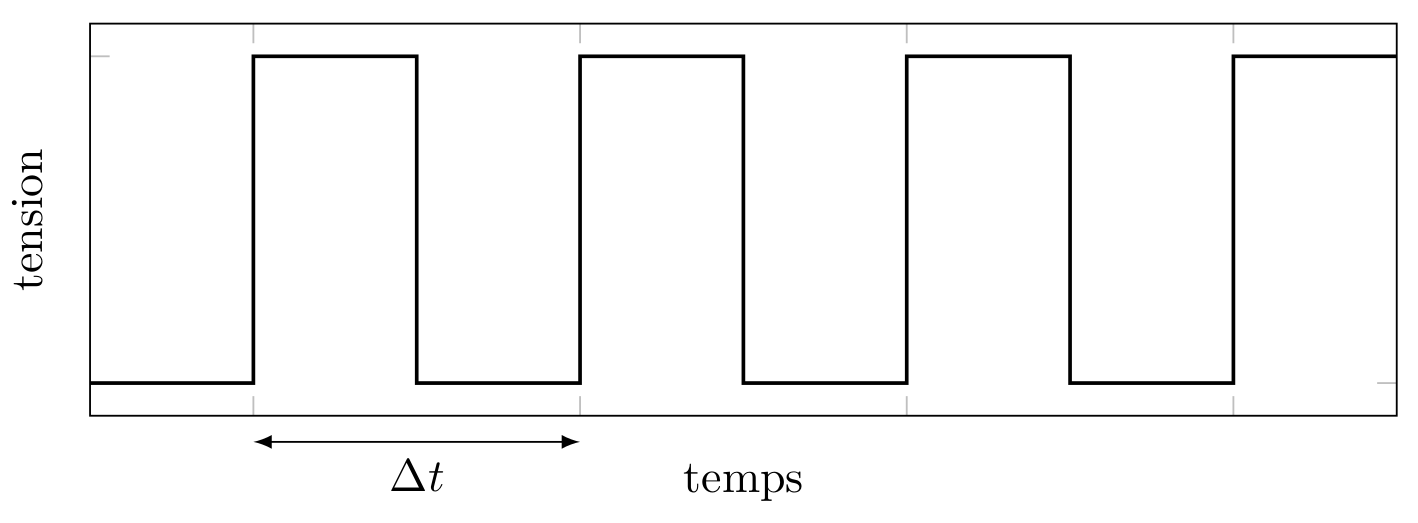
\includegraphics[width=0.5\linewidth]{img/figure_10}
 \caption{Allure du signal de sortie du codeur incrémental}
 \label{img10}
\end{figure}

Une mesure de la vitesse angulaire de rotation de la MCC $\omega_m$, pour une tension de 3.45 V, à partir des données du codeur incrémental est donnée figure \ref{img11}.

\begin{figure}[!h]
\centering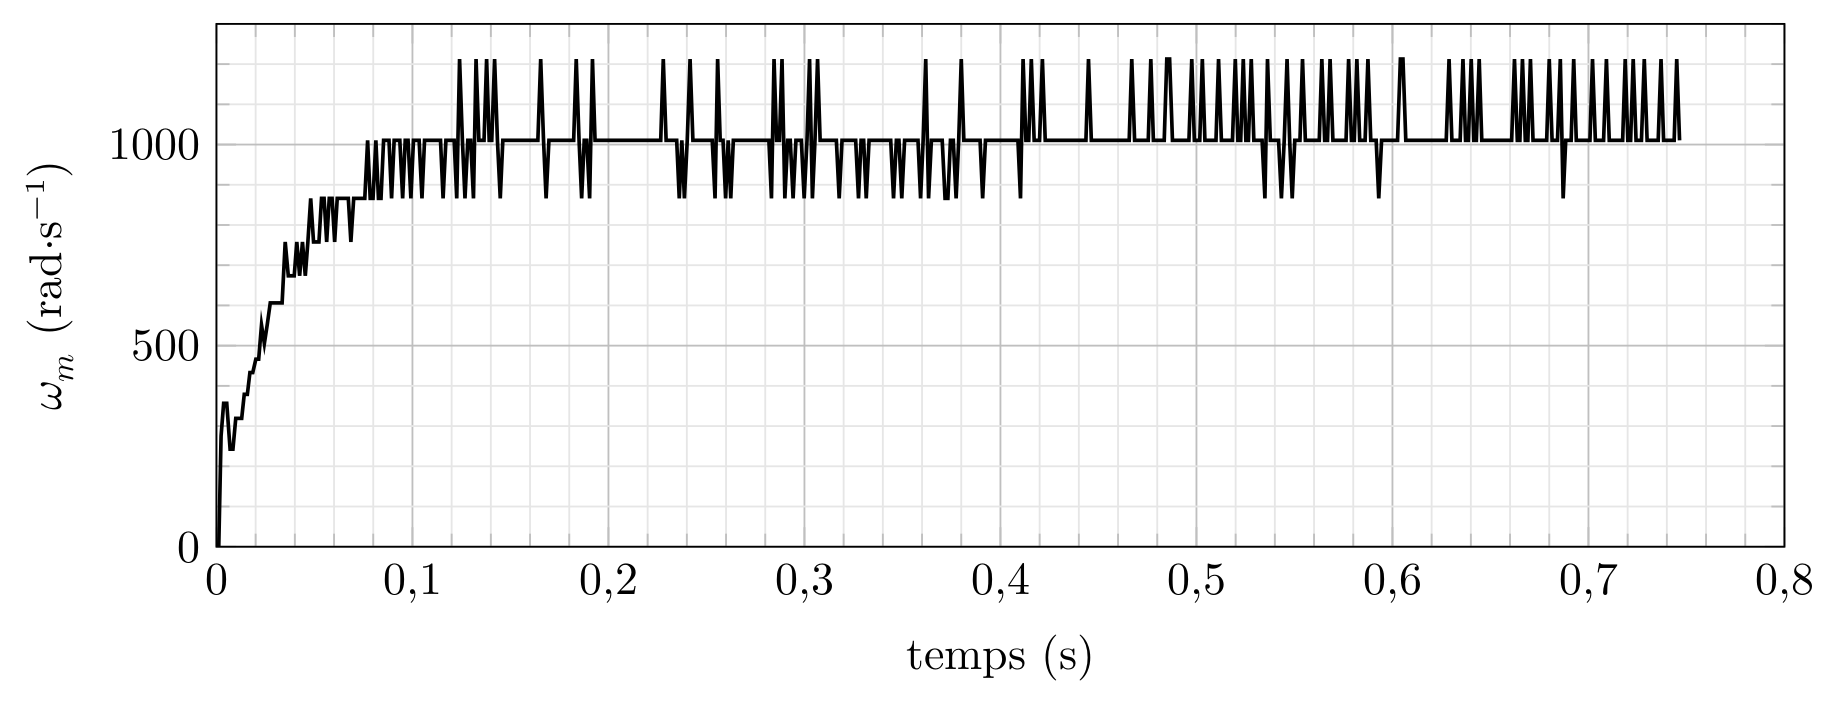
\includegraphics[width=0.9\linewidth]{img/figure_11}
 \caption{Mesure de la vitesse angulaire de rotation moteur $\omega_m$ non filtrée}
 \label{img11}
\end{figure}

Des \og pics\fg\ apparaissent sur la mesure de la vitesse. Afin que ce phénomène n'influe pas le fonctionnement global de l'objectif photographique, un filtre est mis en place.

Sa fonction de transfert est $H(j\omega)=\frac{\Omega_{mf}(j\omega)}{\Omega_{m}(j\omega)}=\frac{H_0}{1+j\frac{\omega}{\omega_0}}$
avec $H_0=1$ et $\omega_0=200rad\cdot s^{-1}$. Ce filtre sera implanté dans un script en Python afin de faciliter l'analyse des mesures.

On montre que la pulsation des pics dus aux impulsions du codeur incrémental est $\omega_{pics}=10800rad.s^{-1}$.

\question{Déterminer le gain en dB de ce filtre pour la fréquence des pics. Justifier alors l'utilisation de ce filtre pour éliminer ces \og pics \fg non désirés.}

Le script en Python permettant d'implanter et d'afficher le résultat du filtre est donné sur le document réponse. On a déterminer l'équation de la récurrence à appliquer : \\
$\omega_{mf}[i+1]=\omega_{mf}[i](1-\omega_0(t_{i+1}-t_i))+H_0(t_{i+1}-t_i)\omega_0\omega_m[i]$

\question{Compléter les lignes 8, 9 et 10 du script Python du document réponse permettant de filtrer les mesures de la vitesse de rotation de la MCC.}

Tous ces résultats sont utilisés pour tracer la courbe de la figure \ref{img12} à partir de plusieurs essais à vide avec des tensions d'induit $u_m$ différentes.

\begin{figure}[!h]
\centering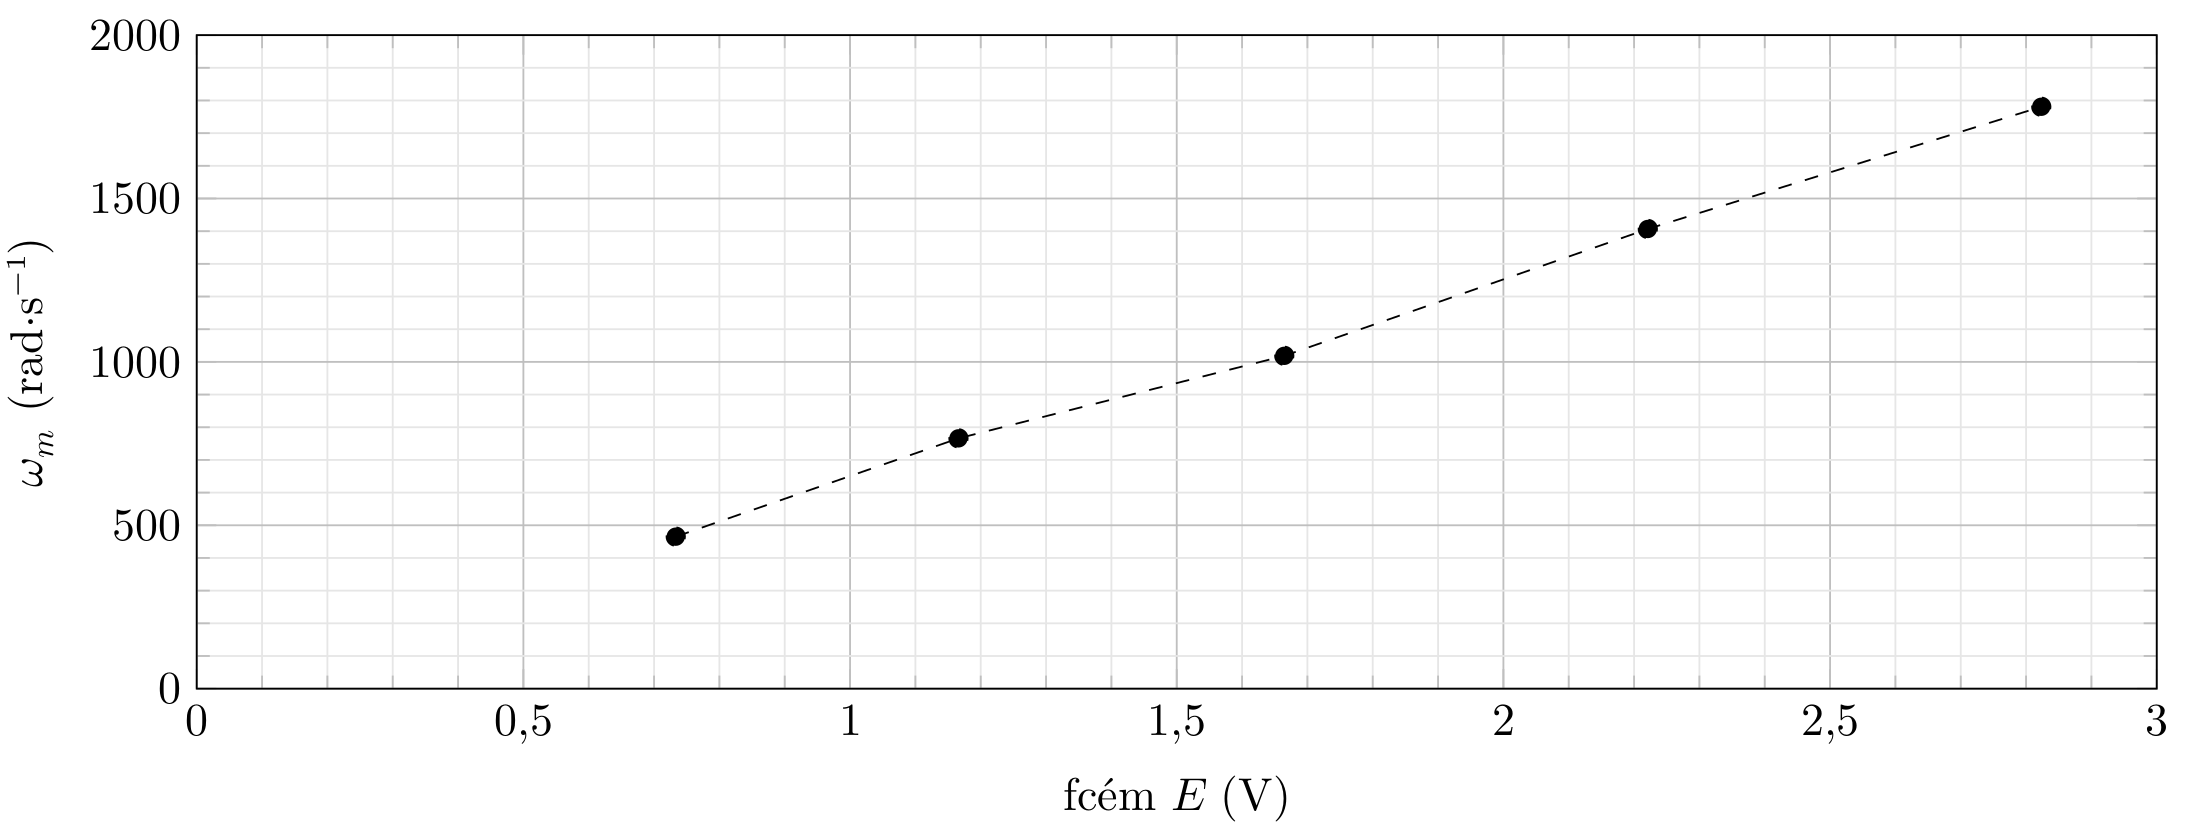
\includegraphics[width=0.9\linewidth]{img/figure_12}
 \caption{Mesures de vitesses angulaire du moteur en régime permanent pour différentes tensions d'induit}
 \label{img12}
\end{figure}

\question{Déterminer à partir de ces résultats la valeur numérique de la constante de force électromotrice $K_e$. En déduire, en la justifiant, la valeur de la constante de couple $K_T$.}

\subsection{Modélisation du frottement}

\paragraph{Objectif}

Modéliser et quantifier les non linéarités liées au frottement

Le réglage de la lentille nécessite un asservissement en position. Dans ce cas le frottement qui induit une non linéarité avec un seuil va perturber le système. Ainsi, il est primordial de quantifier les coefficient pour pouvoir régler la commande. Des essais ont été réalisés sur un prototype pour déterminer les valeurs des couples de frottement sec $C_0$ et visqueux $f$.

Quelle que soit la valeur trouvée précédemment, on prendra pour valeur de la constante de couple $K_T$ de la MCC, $K_T=0.0019 N\cdot m\cdot A^{-1}$.

Différents essais sont effectués pour plusieurs tensions d'alimentation de la MCC. Les résultats sont donnés sur la figure \ref{img13}.

\begin{figure}[!h]
\centering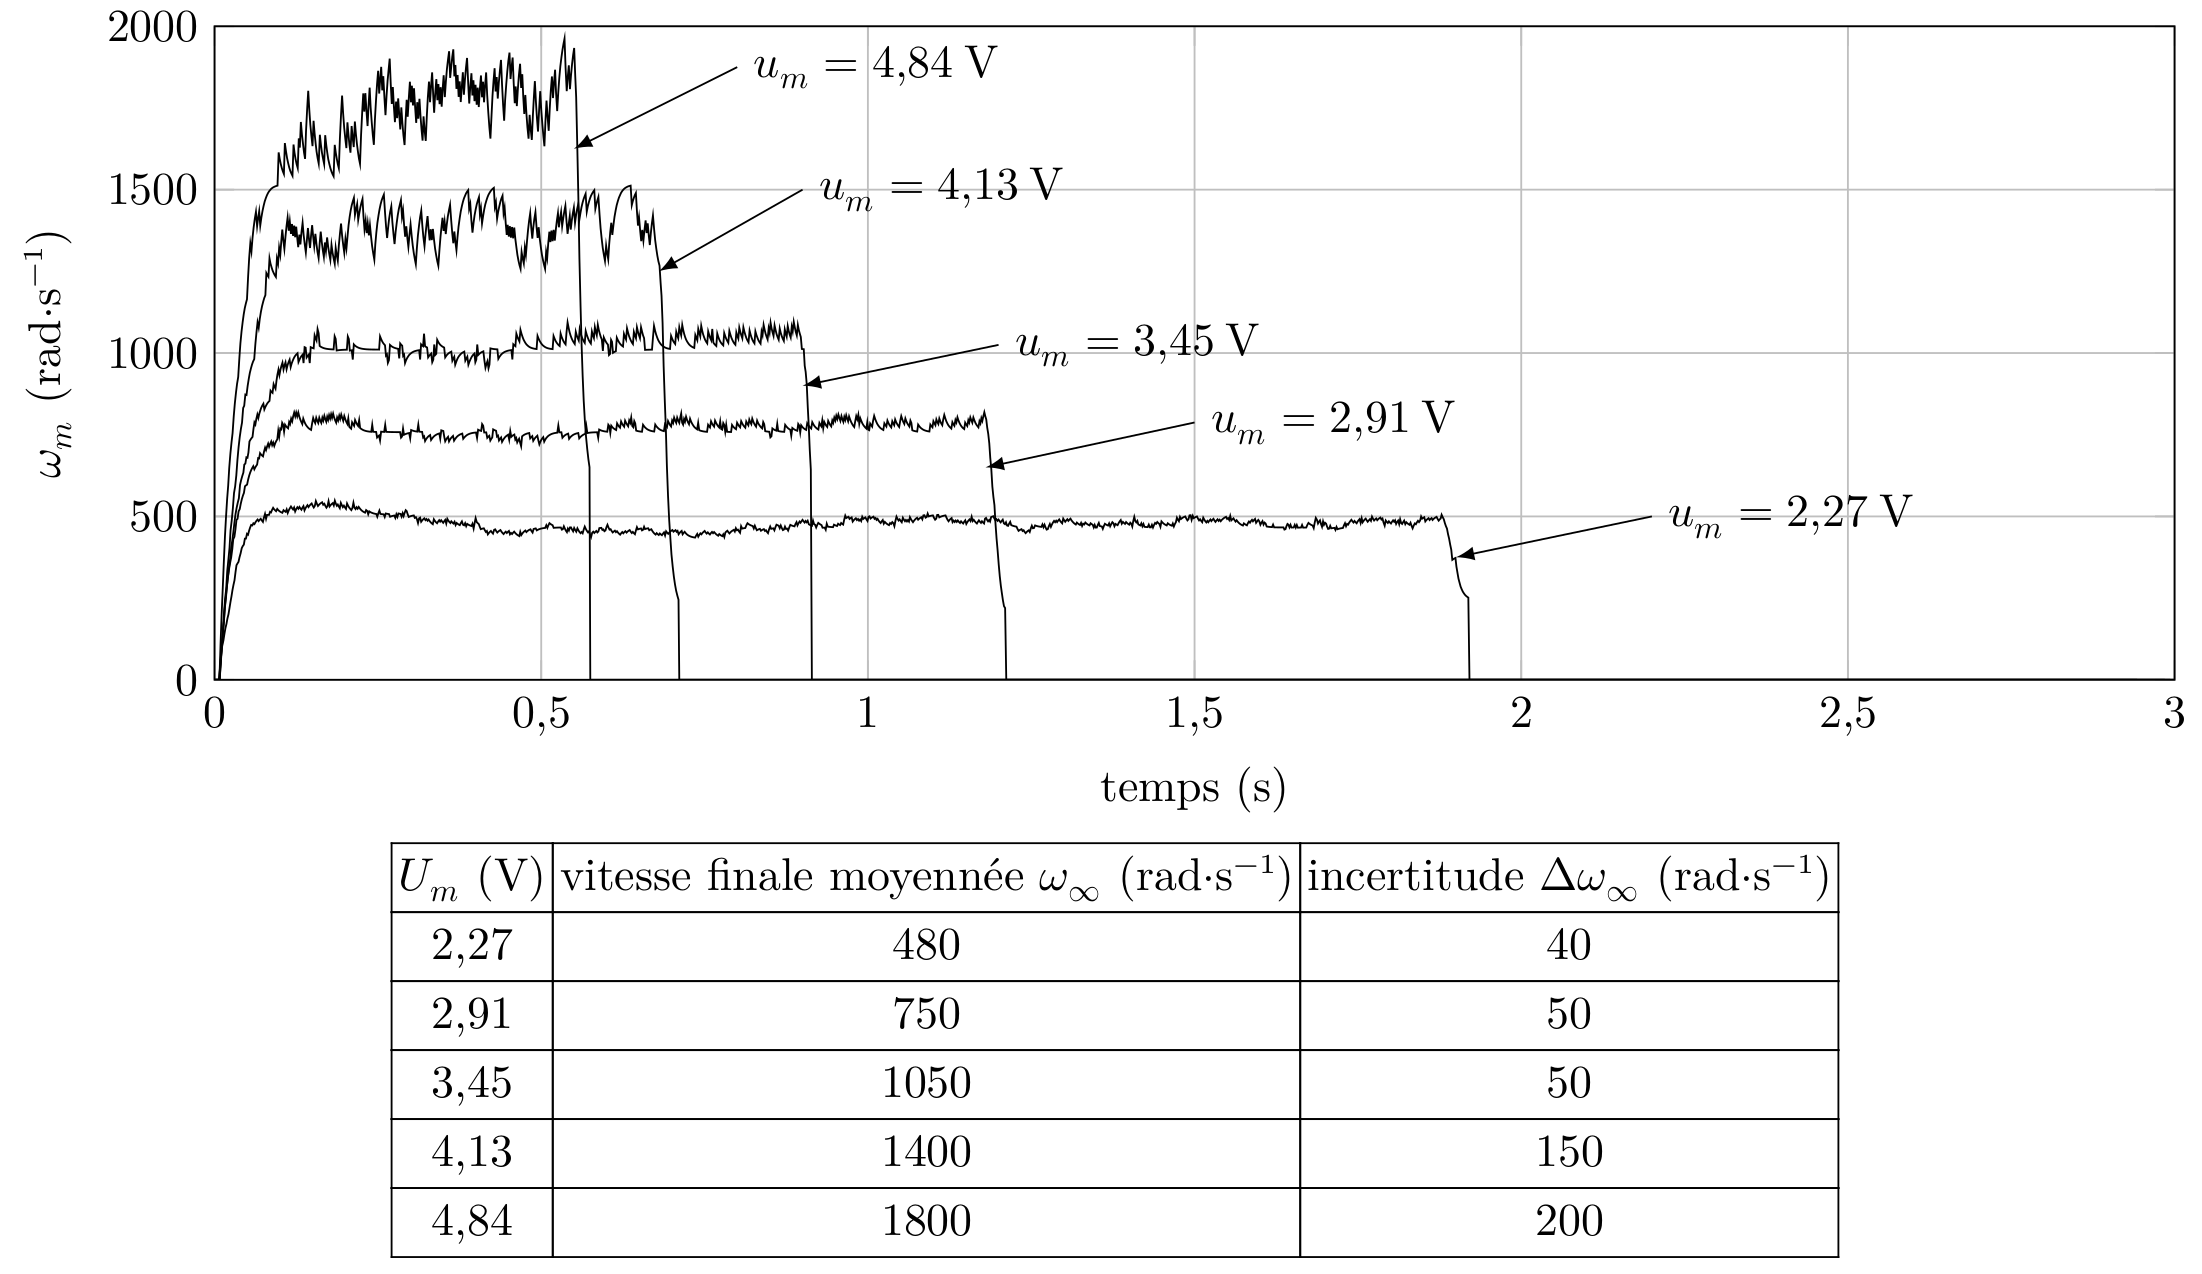
\includegraphics[width=0.9\linewidth]{img/figure_13}
 \caption{Mesures de vitesses angulaire du moteur en régime permanent pour différentes tensions d'induit}
 \label{img13}
\end{figure}

\question{Déterminer l'expression de la vitesse de rotation de la MCC en régime permanent notée $\omega_\infty$ en fonction des paramètres $U_m$, $C_0$, $K_T$, $K_e$, $R_m$ et $f$.}

Le tableau de la figure 13 donne la vitesse en régime permanent $\omega_\infty$ ainsi que l'incertitude sur la mesure $\Delta\omega_\infty$.

\question{Tracer sur le document réponse la courbe $\omega_\infty$ ($U_m$).}

\question{En déduire les valeurs numériques de $C_0$ et $f$.}

%\question{Placer sur la courbe les incertitudes dues à la dispersion des mesures.}

%\question{En tenant compte des incertitudes dans la mesure de vitesse, donner un encadrement de $C_0$ et de $f$.}

\section{Choix et réglage du correcteur permettant de \og gérer le mouvement de l'optique \fg}

\paragraph{Objectif}

Choisir et régler un correcteur afin de répondre aux exigences du cahier des charges.

\begin{center}
\begin{tabular}{|p{7.4cm}|p{4.4cm}|p{3.4cm}|}
\hline
Exigence & Critère d'appréciation & Niveau \\
\hline
\multirow{2}{*}{Id = "1.2.2" Gérer le mouvement de l'optique} & précision, erreur statique & $<0.1\%$\\
\cline{2-3}
& stabilité - marge de phase & 45\textdegree\ mini\\
\cline{2-3}
& rapidité - $t_{r5\%}$ & 0.6s maxi\\
\cline{2-3}
& dépassement - $D_1$ & aucun dépassement\\
\hline
\end{tabular}
\end{center}

Le réglage nécessite un compromis entre les différents critères. Le frottement sec induit une difficulté particulière car il impacte fortement la rapidité : si le gain en boucle ouverte est trop faible le système ne pourra pas se mettre en mouvement, si celui-ci est trop élevé, le système risque de devenir instable. La suite du questionnement
a pour but d'étudier comment trouver un bon compromis.

Le modèle causal de l'objectif photographique dont les paramètres ont été déterminés expérimentalement précédemment est donné figure 14.

\begin{figure}[!h]
\centering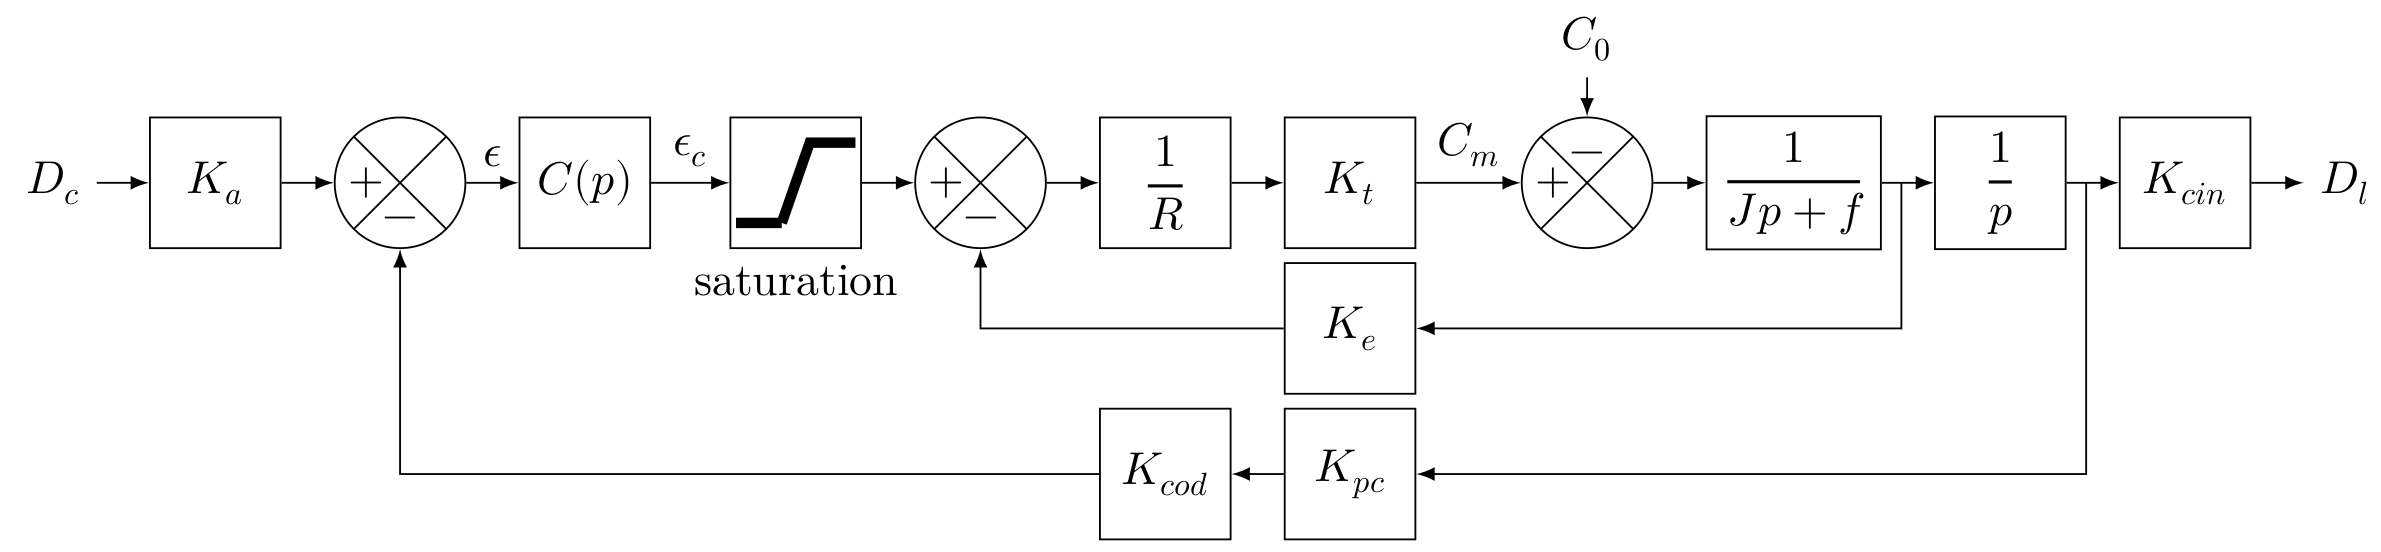
\includegraphics[width=0.9\linewidth]{img/figure_14}
 \caption{Schéma-bloc de l'asservissement de la position de la lentille}
 \label{img14}
\end{figure}

Dans la figure \ref{img14}, le couple de frottement sec est modélisé par un échelon de perturbation. Cette modélisation couramment utilisée présente l'inconvénient de ne pas tenir compte du signe du mouvement et de ne pas avoir de seuil de mouvement. Cette non linéarité peut se décrire de manière plus fine à l'aide d'un bloc bande morte
(figure \ref{img15}) qui permet de modéliser la phase de décollage.

\begin{figure}[!h]
\centering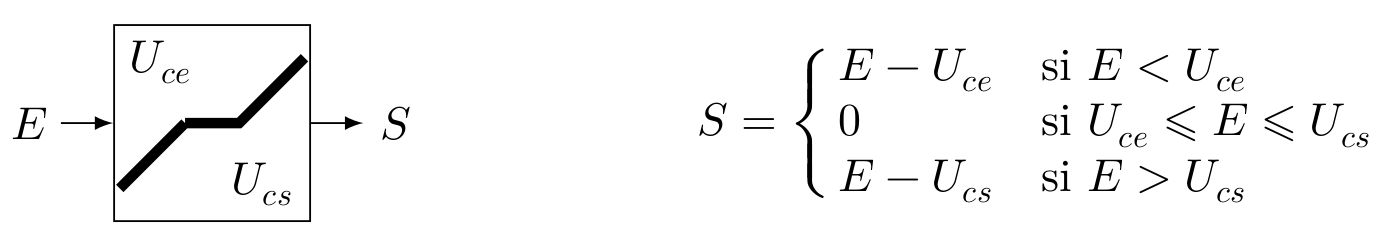
\includegraphics[width=0.6\linewidth]{img/figure_15}
 \caption{Principe d'un bloc bande morte}
 \label{img15}
\end{figure}

\question{Réaliser une fonction python \verb?S(E,Uce,Ucs)? permettant de traduire le fonctionnement de la bande morte.}

Il serait possible de déterminer les bornes de la bande morte en $N\cdot m$. 

Néanmoins, pour le réglage il est beaucoup plus pratique d'observer l'effet de la bande morte au niveau de la commande du moteur. Ainsi toutes les non linéarités sont placées au même endroit. Afin de trouver les bornes de la bande morte au niveau de la commande moteur, il faut déplacer le sommateur afin de le sortir de la boucle (figure \ref{img16}).

\begin{figure}[!h]
\centering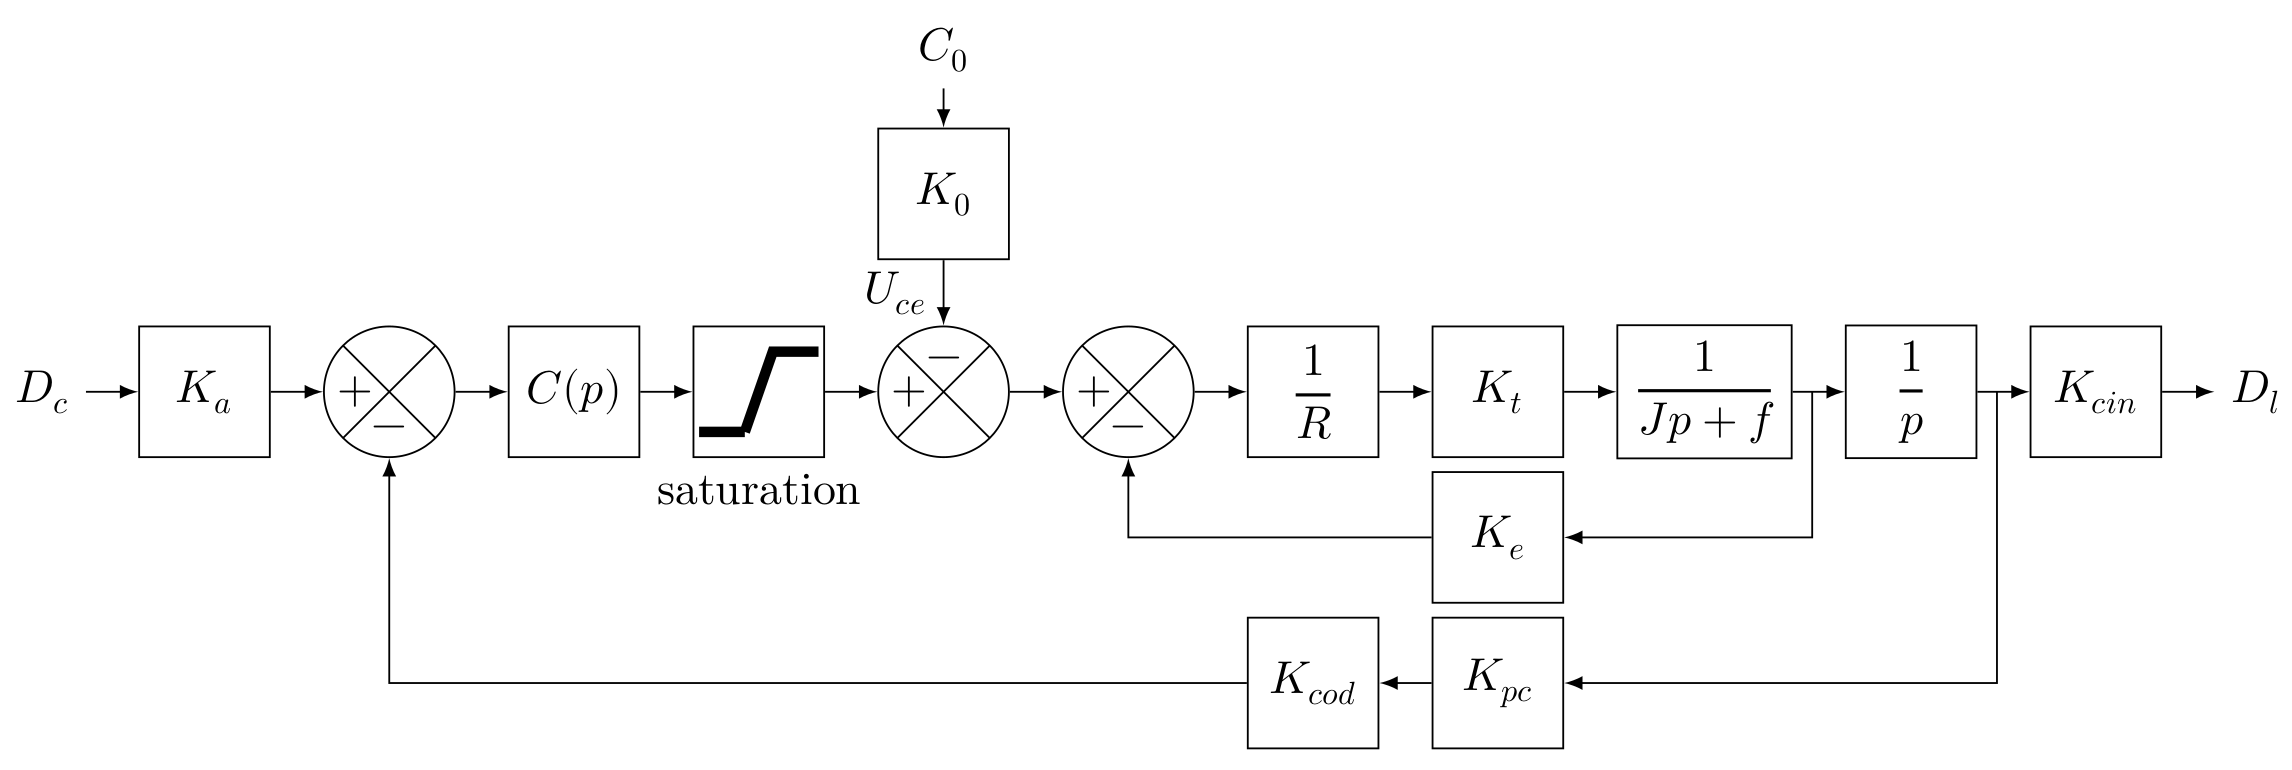
\includegraphics[width=0.9\linewidth]{img/figure_16}
 \caption{Schéma-bloc modifié de l'asservissement de la position de la lentille}
 \label{img16}
\end{figure}

\question{Trouver l'expression de $K_0$ lié au déplacement du sommateur. En déduire la valeur de $U_{ce}=K_0\cdot C_0$.}

Pour la suite on prendra $U_{ce}=1.4V$. Le modèle obtenu est donné figure \ref{img17}.

\begin{figure}[!h]
\centering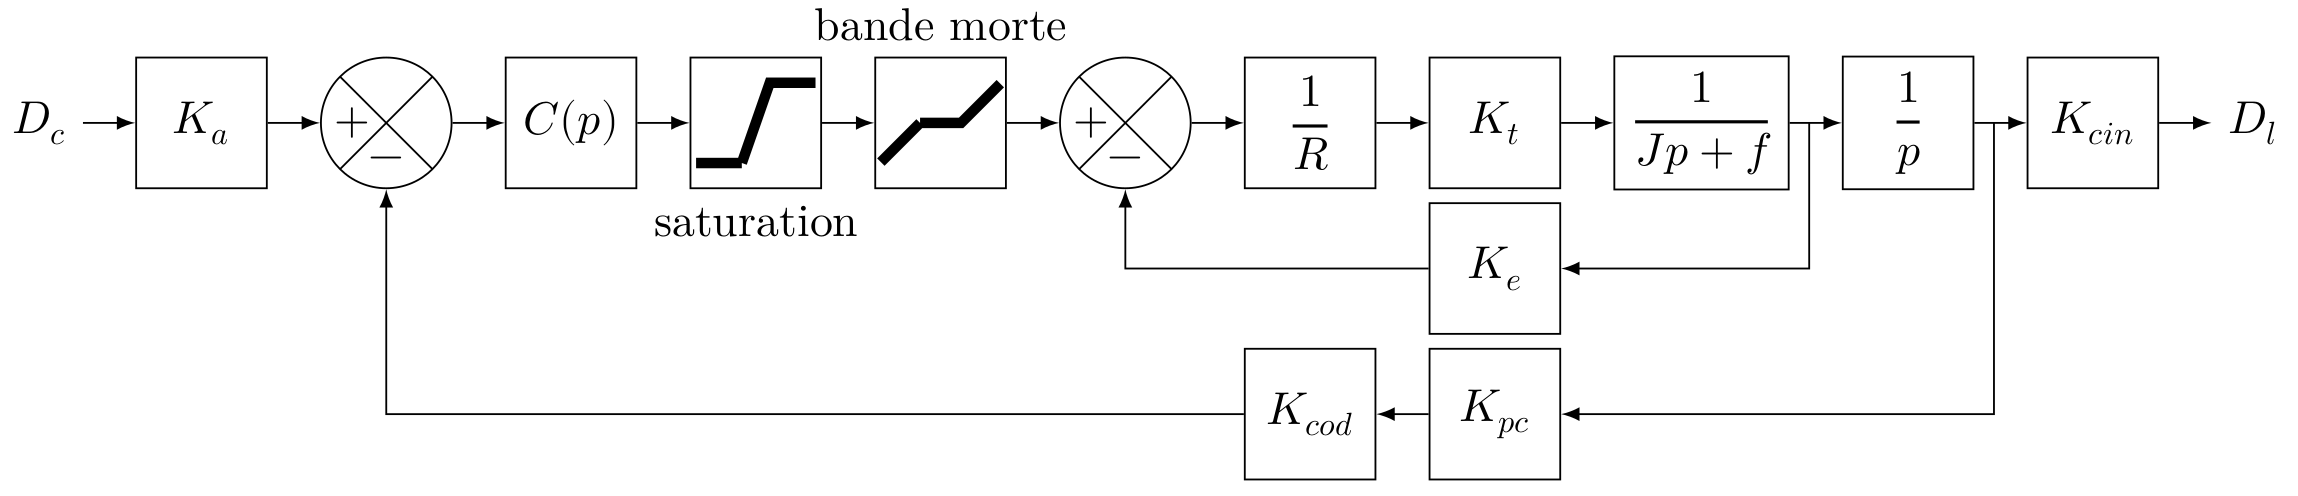
\includegraphics[width=0.9\linewidth]{img/figure_17}
 \caption{Schéma-bloc de l'asservissement de la position de la lentille avec bande morte}
 \label{img17}
\end{figure}

La fonction de transfert de ce correcteur est $C(p)=\frac{\epsilon_c(p)}{\epsilon(p)}=K_p+\frac{K_i}{p}=K_p\cdot\left(1+\frac{1}{\frac{K_p}{k_i}\cdot p}\right)$.


L'utilisation du correcteur proportionnel intégral se justifie pour le critère de précision. En effet, même s'il y a un intégrateur dans la chaine d'action, celui-ci est placé après la perturbation dont l'effet ne sera donc pas annulé.

Le diagramme de Bode de la FTBO du système avec C(p) = 1 est donné figure \ref{img18}.

Remarque : Le diagramme tracé est celui du modèle linéaire qui ne prend pas en compte la bande morte et la saturation. En effet, il n'est pas possible de tracer le diagramme du modèle non linéaire. La conséquence est qu'il n'est pas possible de conclure sur la rapidité à partir de l'analyse harmonique.

\begin{figure}[!h]
\centering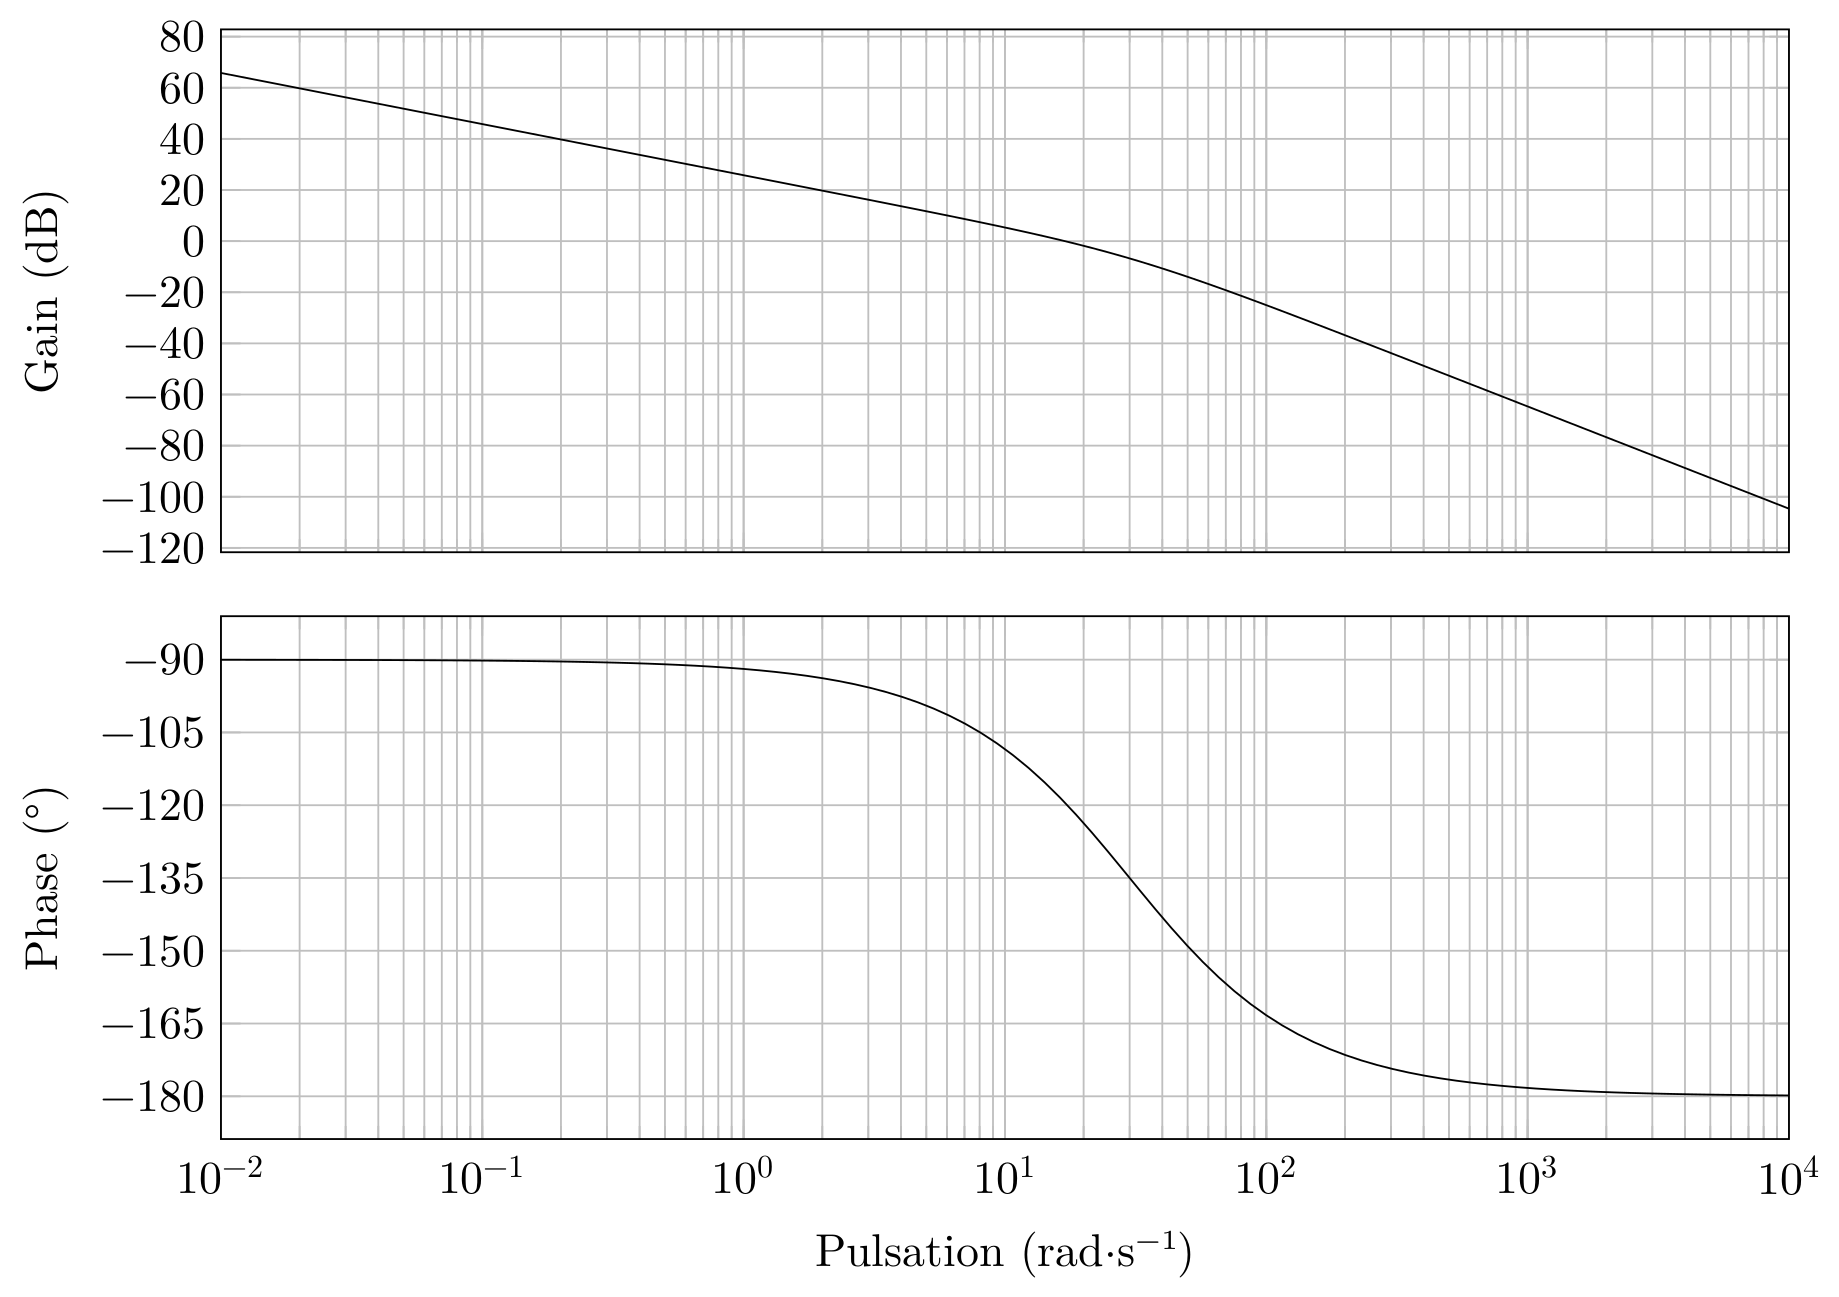
\includegraphics[width=0.9\linewidth]{img/figure_18}
 \caption{Diagramme de Bode en boucle ouverte avec $C(p)=1$}
 \label{img18}
\end{figure}


\question{Déterminer l'expression de la FTBO à partir du diagramme de Bode de la figure \ref{img18}. On donne $10^{\frac{-1}{4}}=0.56$.}

\cleardoublepage

\ifdef{\public}{\pagestyle{documentreponse}}{\pagestyle{correction}}

\reponse{5}{}{
$resolution_{abs}=\frac{c}{2^4}=\frac{6}{16}=375\mu m>100\mu m$, la résolution est insuffisante pour une utilisation normale mais le fait que ce soit un capteur absolu, permet d'utiliser cette information pour initialiser le capteur incrémental.}

\reponse{6}{}{
$\frac{\theta_l}{\theta_m}=(-1)^7.\frac{Z_3\cdot Z_4\cdot Z_5\cdot Z_7\cdot Z_9\cdot Z_{11}\cdot Z_{12}\cdot Z_{14}}{Z_4\cdot Z_5\cdot Z_6\cdot Z_8\cdot Z_{10}\cdot Z_{12}\cdot Z_{13}\cdot Z_{15}}=-
\frac{12\cdot 22\cdot 12\cdot 15\cdot 13 \cdot 11\cdot  39\cdot 10}{22\cdot 12\cdot 26\cdot 28\cdot 25\cdot 39\cdot 27\cdot 100}=-
\frac{11}{14\cdot 5 \cdot 3\cdot 10}=-
\frac{11}{2100}=
-\frac{10.5}{2100}-\frac{0.5}{2100}\approx-0.005-0.00025\approx-0.00525$

$d_l=\frac{p}{2\cdot \pi}\cdot |r|\cdot \theta_{rc}$

Le plus petit angle mesuré est $\theta_{rc}=\frac{2\cdot \pi}{30}$, donc 

$resolution_{inc}=\frac{p}{2\cdot \pi}\cdot |r|\cdot \frac{2\cdot \pi}{30}=30\cdot |r|\cdot \frac{1}{30}=0.00525=5.25\mu m$
}

\reponse{5}{}{Pour coder $6mm$, avec une résolution de $5\mu m$, il faut $resolution=\frac{6}{0.005}=1000\cdot\frac{6}{5}=1200$.

On sait que $2^{10}=1024$ et $2^{11}=2048$, il faut donc $11$bits.}

\ifdef{\public}{\newpage}

\reponse{0}{\begin{center}
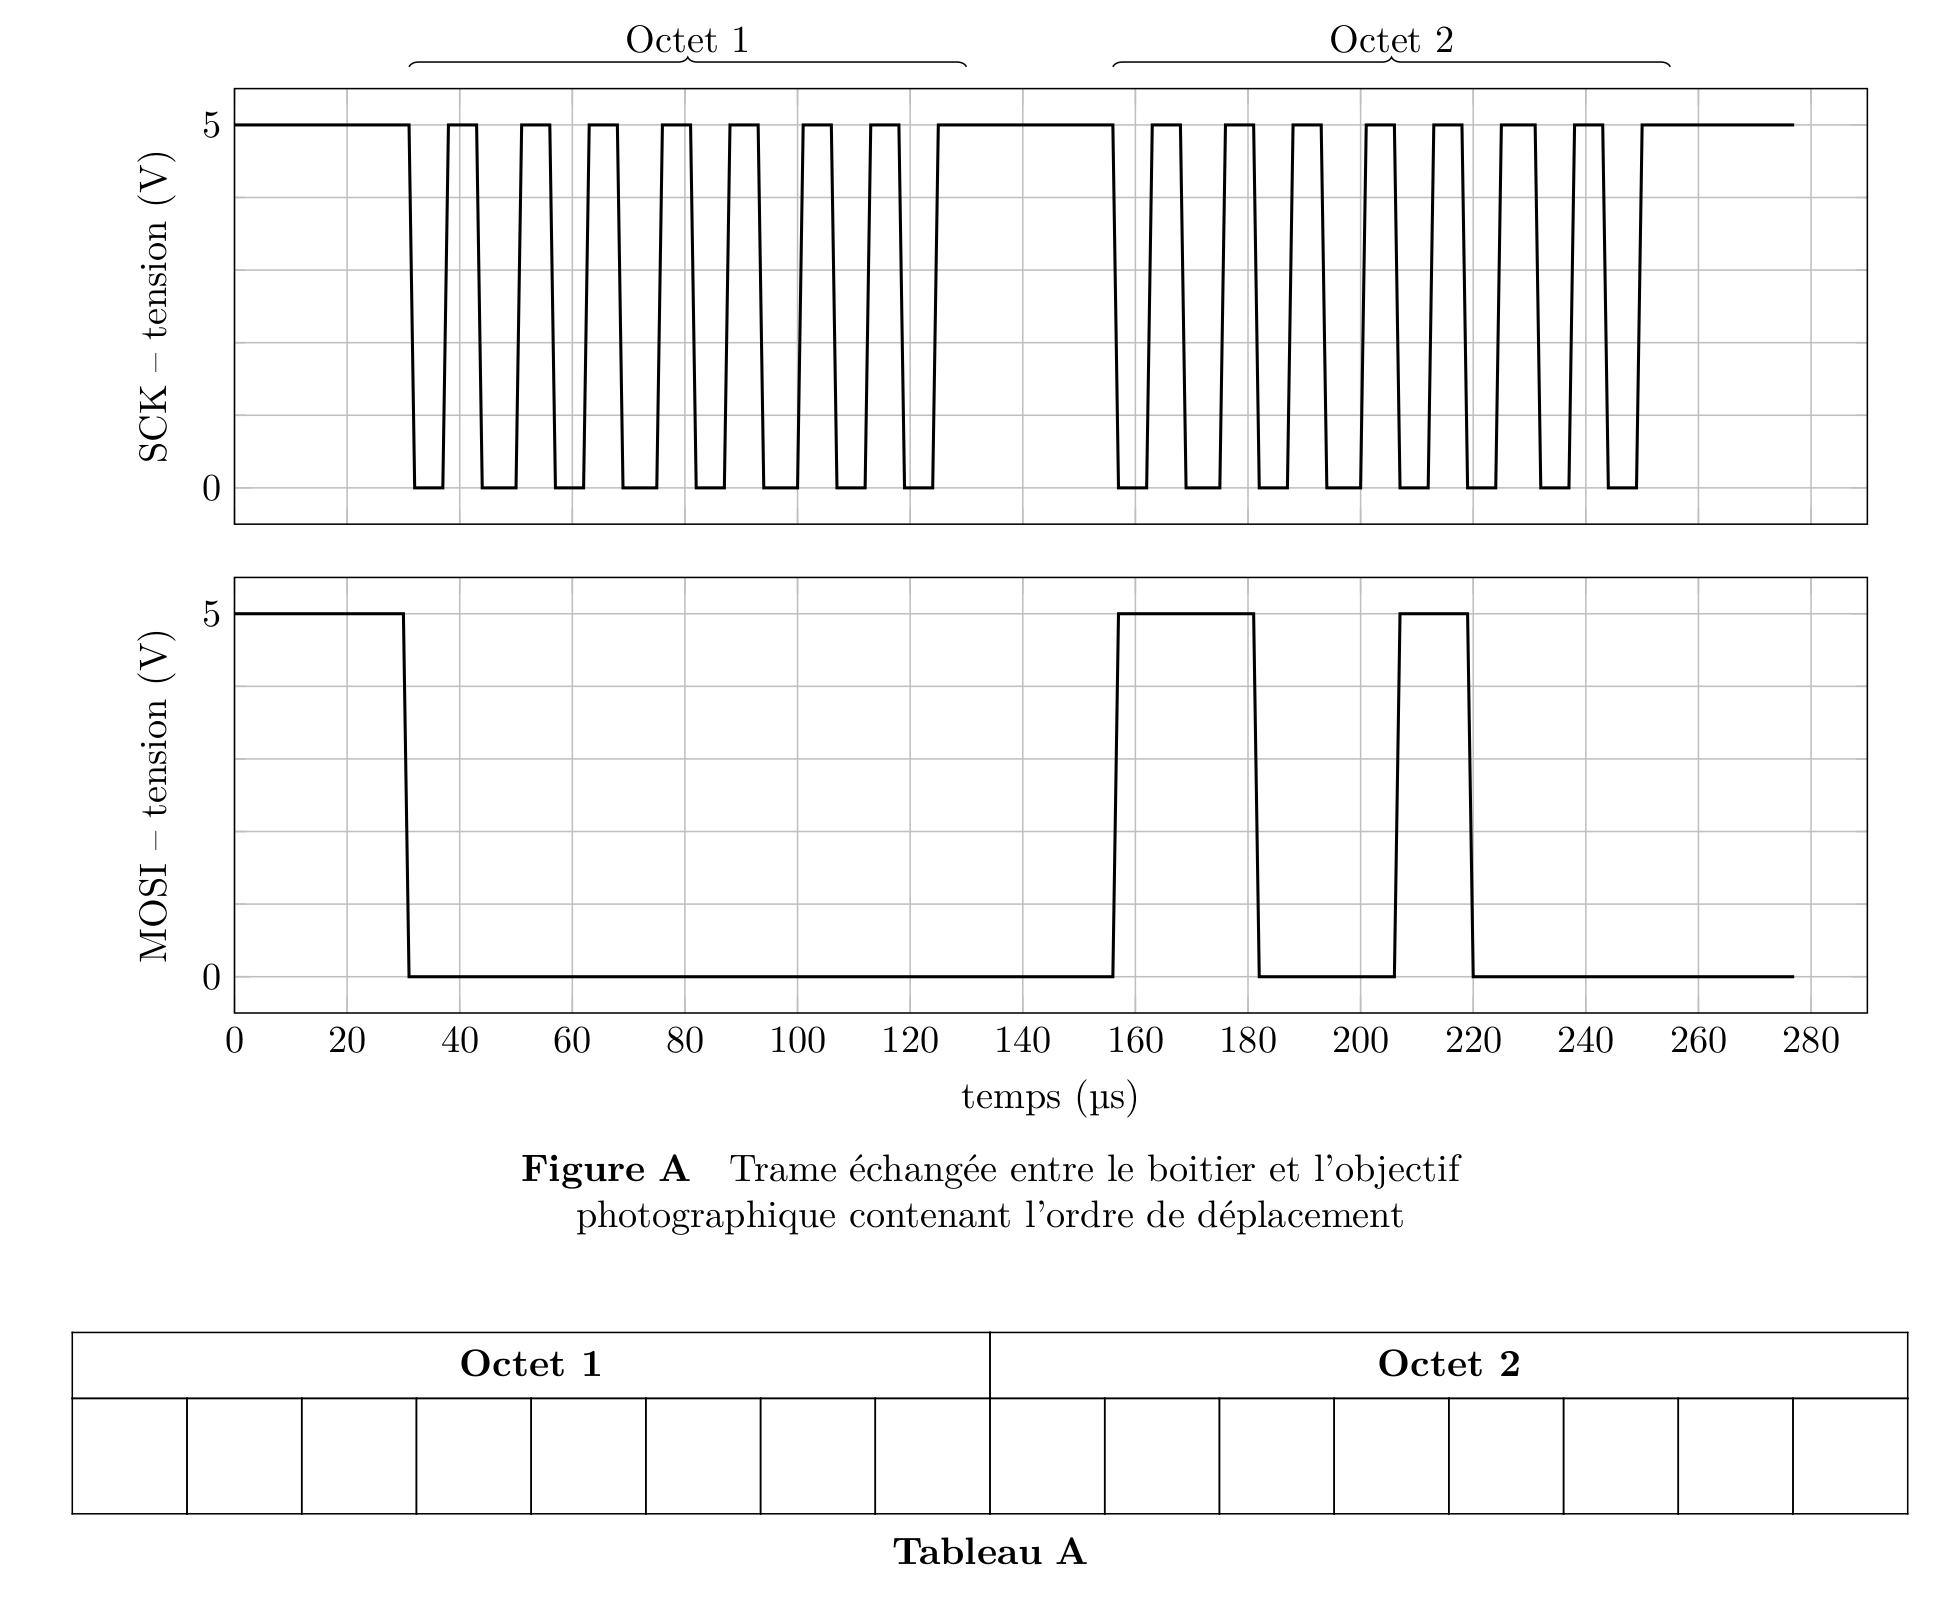
\includegraphics[width=0.7\linewidth]{img/DR_01}
\end{center}\vspace{-1cm}}{
\begin{center}
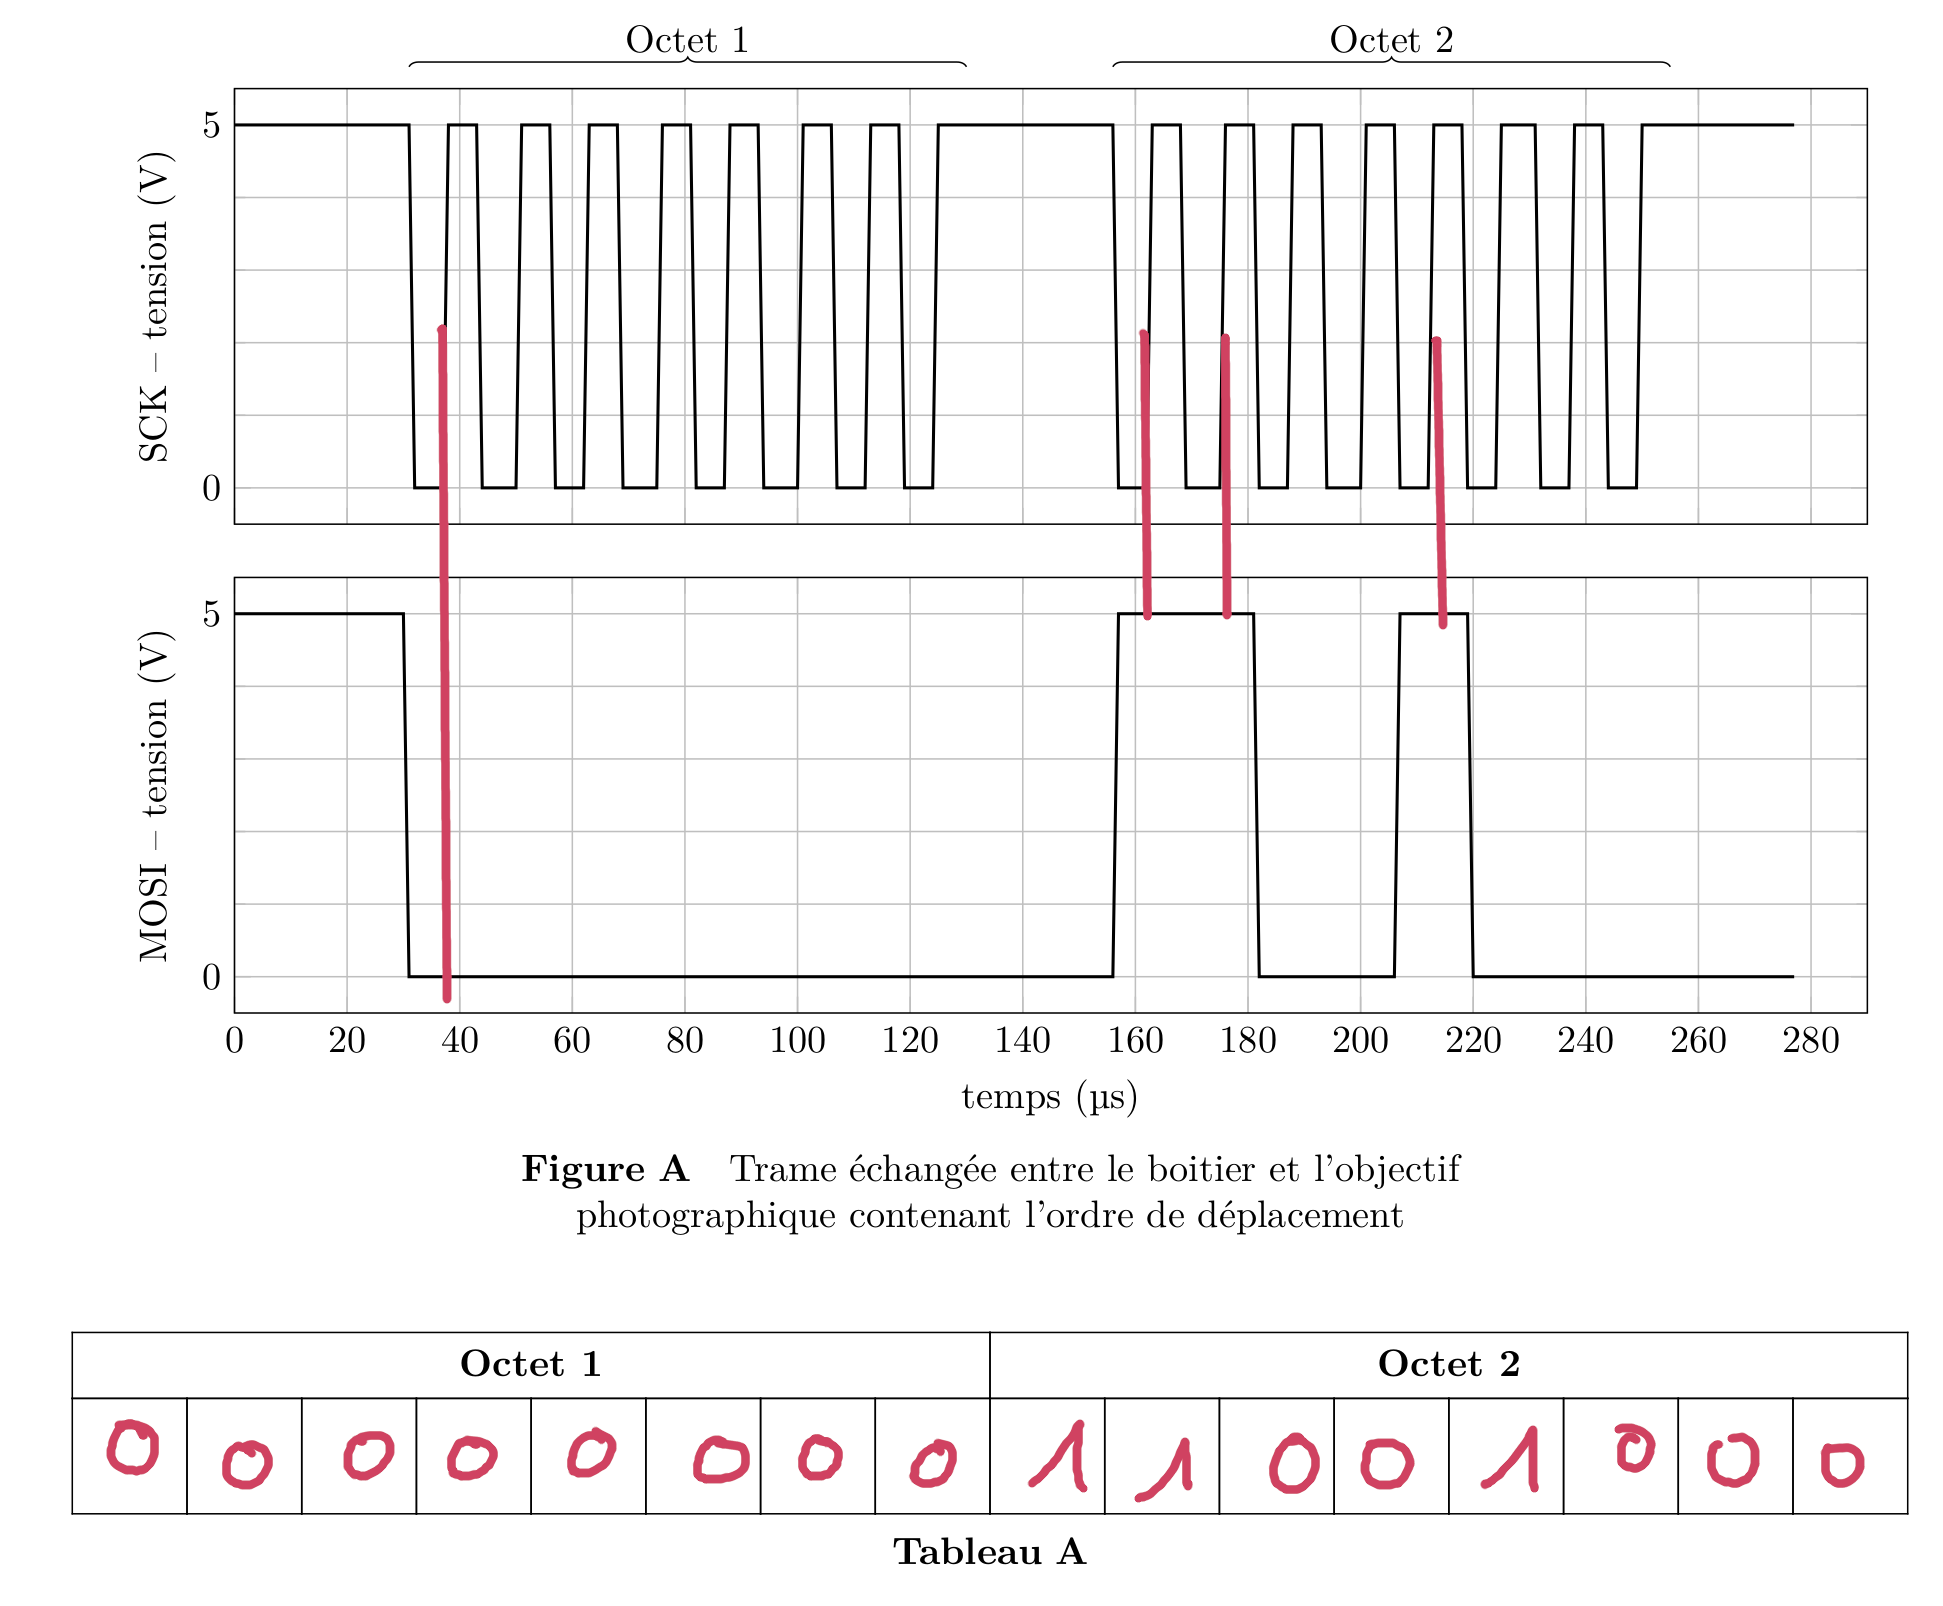
\includegraphics[width=0.7\linewidth]{img/DR_01_cor}
\end{center}}

\reponse{4}{}{On décode donc $a=(11001000)_2=2^7+2^6+2^7+2^3=128+64+8=200$

Le déplacement est donc $d=200\cdot 5\mu m=1mm$.}

\reponse{4}{}{Il faut 3 octets par transmission et la figure du document réponse montre qu'un octet est transmis en $140\mu s$. Il faut donc $420\mu s$ pour une transmission complète et c'est inférieur à $0.5s$.}

\reponse{4}{}{$k=\frac{r\cdot\Phi_1}{\Phi_2}=-0.00525\cdot\frac{2.58}{7.17}\approx-0.005\cdot\frac{2.6}{7.2}\approx-0.005\cdot\frac{1.3}{3.6}\approx-0.005\cdot(\frac{1}{3}+\frac{0.1}{3.6})\approx-0.005\cdot(0.33+0.027)\approx-\frac{0.36}{2\cdot 100}\approx-0.0018$}

\reponse{4}{}{Dans le cycle $0-1-2$, on peut écrire: $\left\{V_{2/0}\right\}=\left\{V_{2/1}\right\}+\left\{V_{1/0}\right\}$


$\left\{V_{2/0}\right\}=\left\{\begin{array}{c}
 \omega_{2/0}\cdot\vec{z}_0 \\
 \vec{0} 
 \end{array}\right\}_E=\left\{\begin{array}{c}
 \omega_{2/0}\cdot\vec{z}_0 \\
 \vec{0} 
 \end{array}\right\}_C$
 $\left\{V_{2/1}\right\}_F=\left\{\begin{array}{c}
 \vec{0} \\
 V_{2/1}\cdot\vec{z}_0 
 \end{array}\right\}_C$
$\left\{V_{1/0}\right\}_C=\left\{\begin{array}{c}
 \omega_{1/0}\cdot\vec{z}_0 \\
 \vec{0} 
 \end{array}\right\}_C$
 
 $\left\{\begin{array}{l}
 0=0\\
 0=0\\
 \omega_{2/0}-\omega_{1/0}=0\\
 0=0\\
 0=0\\
 V_{2/1}=0
 \end{array}\right.$
 
 Dans le cycle $0-2-3$, on peut écrire: $\left\{V_{3/0}\right\}=\left\{V_{3/2}\right\}+\left\{V_{2/0}\right\}$

$\left\{V_{3/0}\right\}_B=\left\{\begin{array}{c}
 \omega_{3/0}\cdot\vec{z}_0 \\
 p\cdot\omega_{3/0}\cdot\vec{z}_0 \\
 \end{array}\right\}_B=\left\{\begin{array}{c}
 \omega_{3/0}\cdot\vec{z}_0 \\
 p\cdot\omega_{3/0}\cdot\vec{z}_0-a\cdot\omega_{3/0}\cdot\vec{y}_0 \\
 \end{array}\right\}_D$
 $\left\{V_{3/2}\right\}_D=\left\{\begin{array}{cc}
 \omega_{3/2x} & V_{3/2x} \\
 \omega_{3/2y} & 0 \\
 \omega_{3/2z} & V_{3/2z} 
 \end{array}\right\}_D$
 $\left\{V_{2/0}\right\}_E=\left\{\begin{array}{c}
 \omega_{2/0}\cdot\vec{z}_0 \\
 \vec{0} 
 \end{array}\right\}_E=\left\{\begin{array}{c}
 \omega_{2/0}\cdot\vec{z}_0 \\
 -c\cdot\omega_{20}\cdot\vec{y}_0
 \end{array}\right\}_D$

 $\left\{\begin{array}{l}
 \omega_{3/2x}=0\\
 \omega_{3/2y}=0\\
 \omega_{3/0}-\omega_{3/2z}-\omega_{2/0}=0\\
 V_{3/2x}=0\\
 -a\cdot\omega_{3/0}+c\cdot\omega_{20}=0\\
 p\cdot\omega_{3/0}-V_{3/2z}=0
 \end{array}\right.$
}

\reponse{0}{
\begin{center}
$\left(\begin{array}{ccccccccc}
0&0&0&0&0&0&0&0&0\\
0&0&0&0&0&0&0&0&0\\
 &0& &0&0&0&0&0&0\\
0&0&0&0&0&0&0&0&0\\
0&0&0&0&0&0&0&0&0\\
0& &0&0&0&0&0&0&0\\
0&0&0&0& &0&0&0&0\\
0&0&0&0&0& &0&0&0\\
0&0& & &0&0& &0&0\\
0&0&0&0&0&0&0& &0\\
0&0& & &0&0&0&0&0\\
0&0&0& &0&0&0&0& \\
\end{array}\right)\cdot
\left(\begin{array}{c}
\omega_{1/0} \\
V_{2/1} \\
\omega_{2/0} \\
\omega_{3/0} \\
\omega_{3/2x} \\
\omega_{3/2y} \\
\omega_{3/2z} \\
V_{3/2x} \\
V_{3/2z}
\end{array}\right)=
\left(\begin{array}{c}
0\\0\\0\\0\\0\\0\\0\\0\\0\\0\\0\\0	
\end{array}\right)
$\end{center}
}{\begin{center}
$\left(\begin{array}{ccccccccc}
0&0&0&0&0&0&0&0&0\\
0&0&0&0&0&0&0&0&0\\
-1&0&1&0&0&0&0&0&0\\
0&0&0&0&0&0&0&0&0\\
0&0&0&0&0&0&0&0&0\\
0&1&0&0&0&0&0&0&0\\
0&0&0&0&1&0&0&0&0\\
0&0&0&0&0&1&0&0&0\\
0&0&-1&1&0&0&-1&0&0\\
0&0&0&0&0&0&0&1&0\\
0&0&c&-a&0&0&0&0&0\\
0&0&0&p&0&0&0&0&-1\\
\end{array}\right)\cdot
\left(\begin{array}{c}
\omega_{1/0} \\
V_{2/1} \\
\omega_{2/0} \\
\omega_{3/0} \\
\omega_{3/2x} \\
\omega_{3/2y} \\
\omega_{3/2z} \\
V_{3/2x} \\
V_{3/2z}
\end{array}\right)=
\left(\begin{array}{c}
0\\0\\0\\0\\0\\0\\0\\0\\0\\0\\0\\0	
\end{array}\right)
$\end{center}}

\ifdef{\public}{\newpage}

\reponse{6}{}{Il y a 4 lignes remplies de 0 et 8 lignes indépendantes, le rang de la matrice est donc 8.

La mobilité du système est $m=I_c-rg(A)=9-8=1$, il y a donc une mobilité dans ce système.}

\reponse{5}{}{Le degré d'hyperstatisme est $h=6\cdot\gamma-I_c+m=12-9+1=4$. On retrouve les 4 lignes de zéro.}

\reponse{5}{}{Afin de libérer des degrés d'hyperstatisme sur ces liaisons, il faut supprimer des degrés de liaison en rotation autour de $\vec{x}$ et $\vec{y}$, on peut donc remplacer les liaisons 1/0 et 2/3 par des rotules. On peut encore enlever un degré de liaison en transformant une des deux liaisons en linéaire annulaire.}

\ifdef{\public}{\newpage}

\reponse{5}{}{\begin{center}
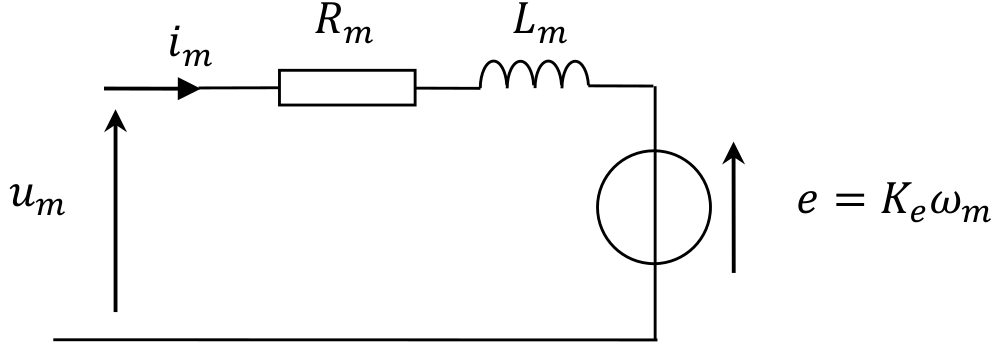
\includegraphics[width=0.5\linewidth]{img/image_03}
\end{center}

Les équations sont les suivantes:
\begin{itemize}
 \item $u_m=e+R_m\cdot i_m+L_m\cdot\frac{di_m}{dt}$,
 \item $e=K_e\cdot \omega_m$,
 \item $C_m=K_T\cdot i_m$.
\end{itemize}

Il faut aussi utiliser la formule donnée dans le sujet:

$C_m-C_0=J\cdot\dfrac{d\omega_m}{dt}+f\cdot\omega_m$.}

\reponse{6}{}{L'essai se faisant à rotor bloqué, on a $\omega_m=0$, ainsi:

$u_m=R_m\cdot i_m+L_m\cdot\frac{di_m}{dt}$

En passant cette équation dans le domaine de Laplace, on trouve:

$U_m=R_m\cdot I_m+L_m\cdot p\cdot I_m$

$\frac{I_m}{U_m}=\frac{1}{R_m+L_m\cdot p}=\frac{\frac{1}{R_m}}{1+\frac{L_m}{R_m}\cdot p}$

On sait que $u_m=1.6V$, ainsi, la courbe peut être vue comme celle de la réponse d'un premier ordre, avec un gain $G=\frac{1}{R_m}$ et une constante de temps $\tau=\frac{L_m}{R_m}$.

On lit sur la courbe la valeur à l'infini: $i_m(+\infty)=75mA=\frac{u_m}{R_m}$, donc $R_m=\frac{1.6}{0.075}\approx 20\Omega$

Par lecture graphique, on trouve $\tau=100-50=50\mu s=\frac{L_m}{20}$, donc $L_m=50\cdot 20=1mH$.
}

\reponse{4}{}{Il y a 30 impulsions par tour, donc le temps entre deux impulsions vaut:

$\Delta_t=\frac{2\cdot \pi}{30\cdot \omega_{rc}}=\frac{2\cdot \pi\cdot \Phi_2}{30\cdot \Phi_1}\cdot\frac{1}{\omega_{m}}$}

\ifdef{\public}{\newpage}


\reponse{5}{}{$20\cdot log\left(\left|H(j\cdot \omega_{pics})\right|\right)=20\cdot log\left(\left|\frac{H_0}{1+j\frac{\omega_{pics}}{\omega_0}}\right|\right)=20\cdot log\left(\left|\frac{1}{1+j\frac{10800}{200}}\right|\right)=20\cdot log\left(\left|\frac{1}{1+j\cdot 54}\right|\right)=-20\cdot.log\left(\left|1+j\cdot 54\right|\right)=-20\cdot log(\sqrt{1+54^2})\approx-20\cdot log(54)\approx-20\cdot(log(100)-log(2))\approx-20\cdot(2-0.3)\approx-20\cdot 1.7\approx-34dB$

Cela signifie que ce filtre va atténuer de 34dB les effets des pics.
}

\refstepcounter{num_rep}
\noindent
\rule{\linewidth}{.5pt}\\
\textbf{Question \ref{\arabic{num_rep}}:} ~\ \\

\begin{lstlisting}[escapeinside={(*}{*)},language=Python]
import matplotlib.pyplot as plt
Omega_m =[0, ..., 1010] # liste des valeurs de la vitesse de rotation mesuree
Temps =[0, ..., 0.83] # amplification statique du filtre
H0=1.0
w0=200 # pulsation de coupure du filtre
Omega_m_f = [Omega_m[0]] # liste des valeurs de la vitesse de rotation filtree
# dt est l'intervalle de temps entre deux valeurs successives dans la liste Temps
for i in range((*\ifdef{\public}{\ \ \ \ \ \ \ \ \ \ \ \ \ \ \ \ \ \ \ }{len(Temps)-1}*)):
dt = (*\ifdef{\public}{}{Temps[i+1]-Temps[i]}*)
omegam_f = (*\ifdef{\public}{}{Omega\_m\_f[i]*(1-dt*w0)+H0*w0*dt*Omega\_m[i]}*)
Omega_m_f.append(omegam_f)
plt.figure(1)
plt.plot(Temps, Omega_m, 'r')
plt.plot(Temps, Omega_m_f)
plt.xlabel("temps en s")
plt.ylabel("vitesse de rotation de la MCC wm rad.s-1")
plt.legend(['Mesure non filtree', 'Mesure filtree'])
plt.show()
\end{lstlisting}

\reponse{4}{}{On assimile la courbe à une droite dont on va identifier la pente en prenant les points extrêmes.

$K_E=\frac{2.82-0.72}{1800-500}=\frac{2.1}{1300}=\frac{21}{13}\cdot 10^{-3}=(1+\frac{8}{13})\cdot 10^{-3}\approx 1.7mV$

Dans le cas du moteur à courant continu, on peut considérer que $K_E=K_T$.}

\ifdef{\public}{\newpage}


\reponse{4}{}{On sait que 

$J\cdot\dfrac{d\omega_m}{dt}=C_m-C_0-f\cdot\omega_m$, ainsi en régime établi:

$C_m-C_0-f\cdot\omega_m=0$, puis $K_T\cdot i_m-C_0-f\cdot\omega_m=0$

De plus, $u_m=e+R_m\cdot i_m+L_m\cdot\frac{di_m}{dt}$, soit en régime établi:

$u_m=e+R_m\cdot i_m$ puis $u_m=K_E\cdot\omega_m+R_m\cdot i_m$

$K_T\cdot \frac{u_m-K_E\cdot\omega_m}{R_m}-C_0-f\cdot\omega_m=0$

$\omega_m\cdot(\frac{K_T\cdot K_E}{R_m}+f)=\frac{K_T}{R_m}\cdot u_m-C_0$

$\omega_m=\frac{K_T}{K_T\cdot K_E +f\cdot R_m}\cdot u_m-\frac{R_m}{K_T\cdot K_E +f\cdot R_m}\cdot C_0$
}

\reponse{0}{\begin{center}
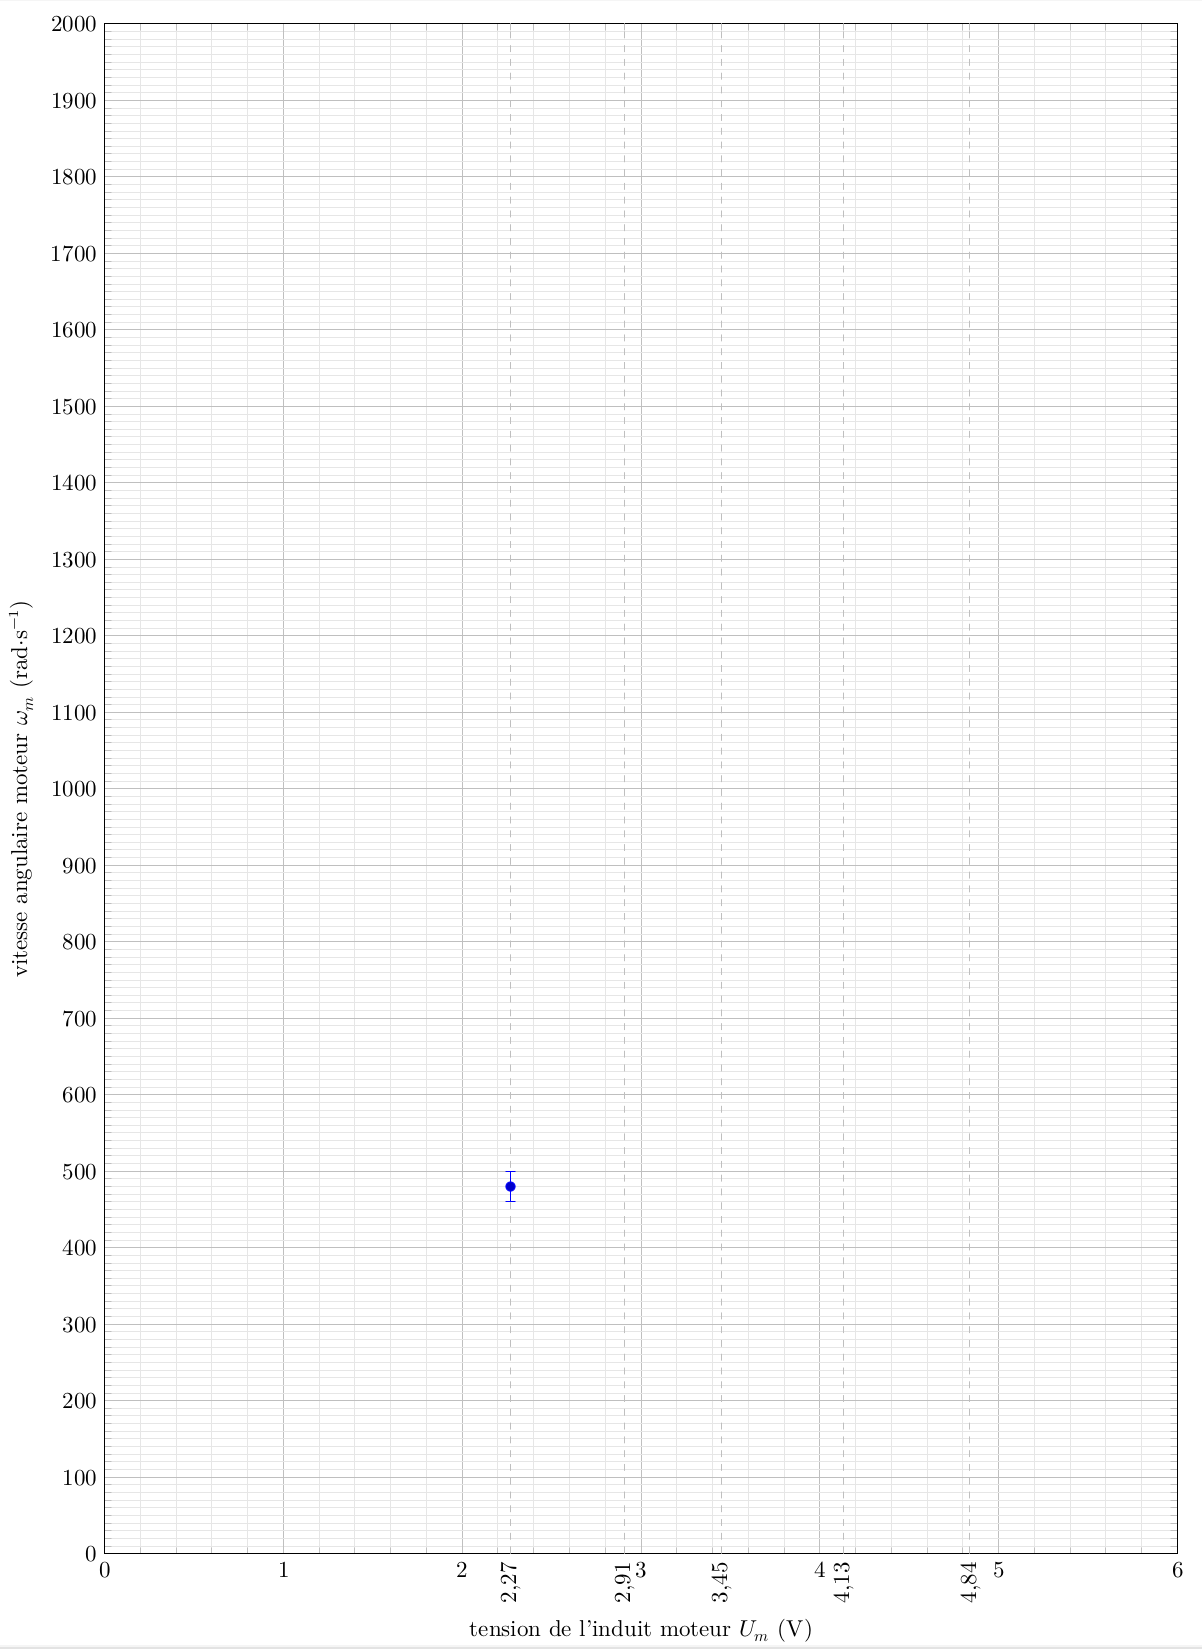
\includegraphics[width=0.7\linewidth]{img/DR_02}
\end{center}\vspace{-1cm}}{
\begin{center}
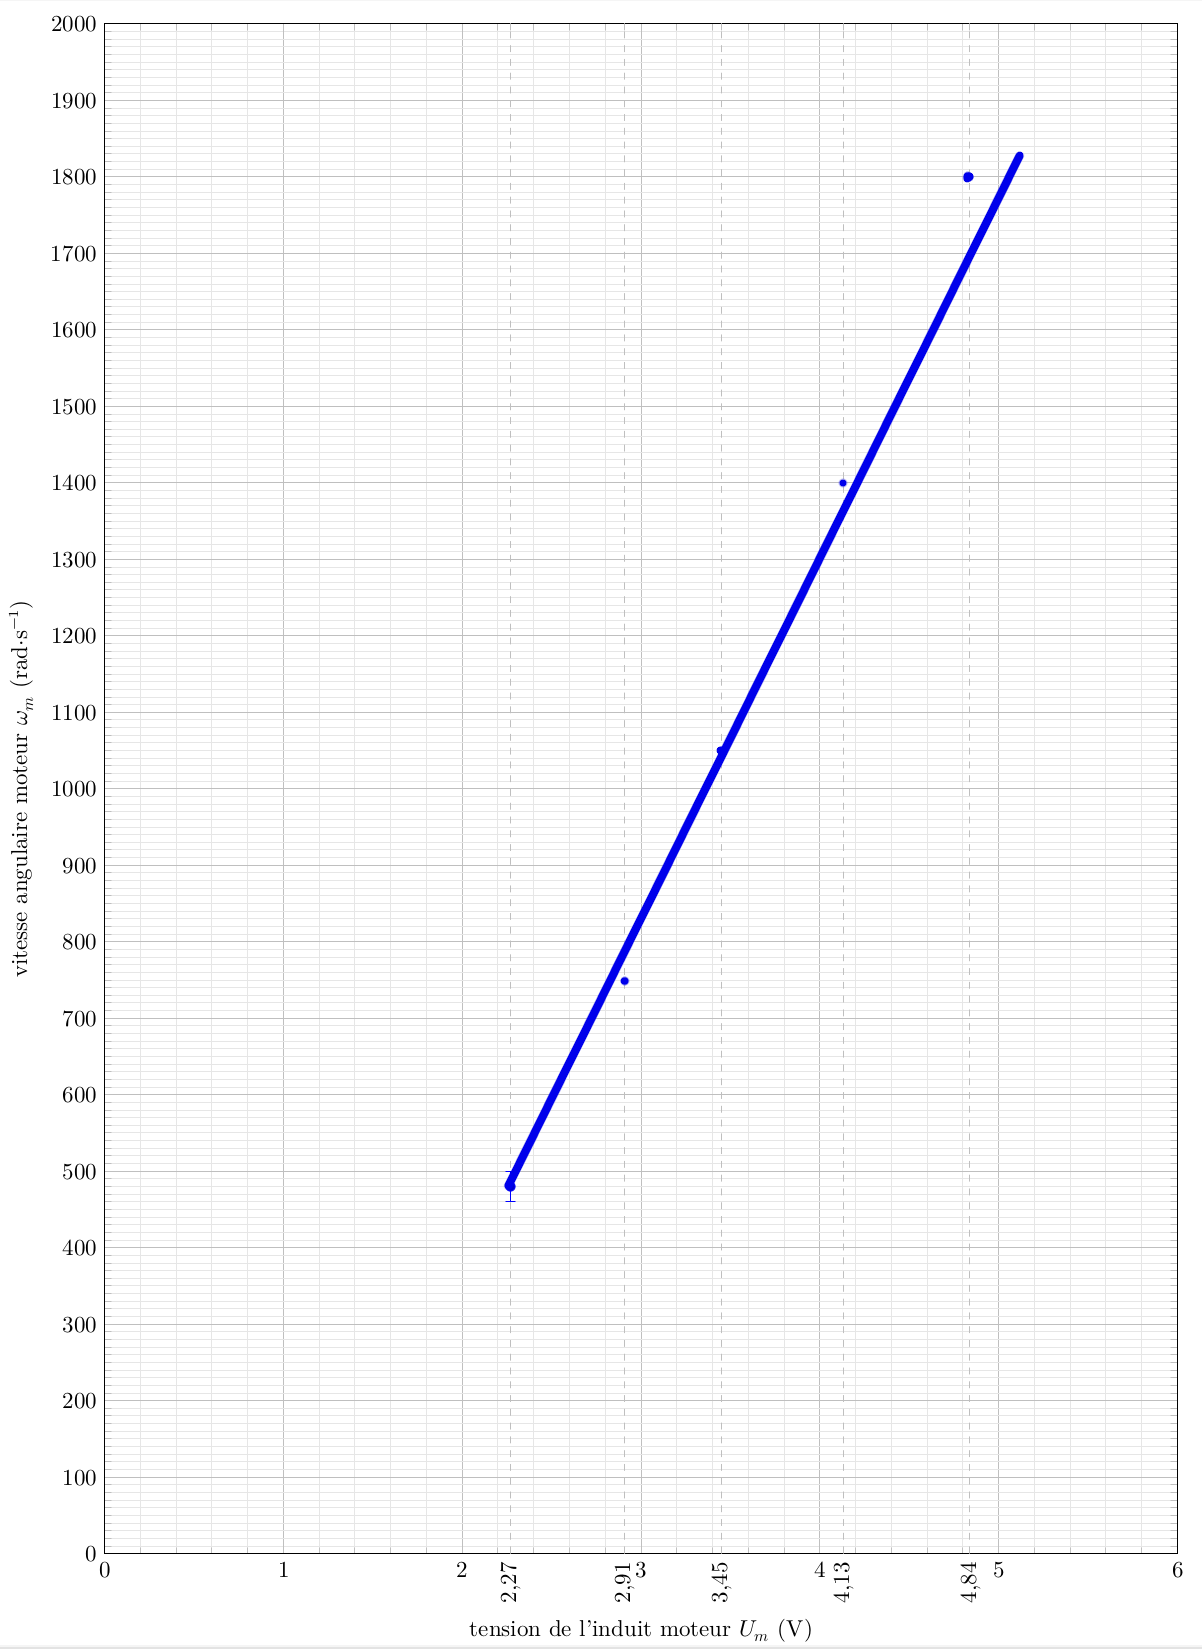
\includegraphics[width=0.7\linewidth]{img/DR_02_cor}
\end{center}}

\reponse{5}{}{L'incertitude étant beaucoup plus faible sur les premiers points, ce sont eux que l'on va choisir pour déterminer l'équation de la droite:

$\frac{1050-480}{3.45-2.27}=\frac{570}{1.18}\approx\frac{570}{1.2}\approx\frac{190}{0.4}\approx\frac{1900}{4}\approx 475$

Donc $\frac{K_T}{K_T\cdot K_E +f\cdot R_m}=475$

$\frac{1.7\cdot 10^{-3}}{1.7\cdot 10^{-3}\cdot 1.7\cdot 10^{-3} +f\cdot 20}=475$

$1.7\cdot 10^{-3}=475\cdot(1.7\cdot 10^{-3}\cdot 1.7\cdot 10^{-3} +f\cdot 20)$

$1.7\cdot 10^{-3}-475\cdot1.7\cdot 10^{-3}\cdot 1.7\cdot 10^{-3}=f\cdot 20\cdot 475$

$f=\frac{1.7\cdot 10^{-3}-0.8\cdot 1.7\cdot 10^{-3}}{20\cdot 475}=\frac{0.2\cdot1.7\cdot 10^{-3}}{20\cdot 475}=\frac{17\cdot 10^{-8}}{4.750}=4\cdot 10^{-8}N\cdot m\cdot rad^{-1}\cdot s$

$480=475\cdot 2.27-\frac{R_m}{K_T\cdot K_E +f\cdot R_m}\cdot C_0$

$\frac{R_m}{K_T\cdot K_E +f\cdot R_m}\cdot C_0=475\cdot 2.27-480$

$C_0=600\cdot \frac{K_T\cdot K_E +f\cdot R_m}{R_m}\cdot $

$C_0=600\cdot \frac{1.7\cdot 10^{-3}\cdot 1.7\cdot 10^{-3} +4\cdot 10^{-8}\cdot 20}{20} $

$C_0=600\cdot \frac{2.9\cdot 10^{-6}+0.8\cdot 10^{-6}}{20} $

$C_0=600\cdot \frac{3.7\cdot 10^{-6}}{20}$

$C_0=600\cdot 1.8\cdot 10^{-7}$
$C_0=0.12\cdot 10^{-3}=0.12mN\cdot m$
}


\refstepcounter{num_rep}
\noindent
\rule{\linewidth}{.5pt}\\
\textbf{Question \ref{\arabic{num_rep}}:} ~\ \\

\begin{lstlisting}[escapeinside={(*}{*)},language=Python]
(*\ifdef{\public}{}{def S(E,Uce,Ucs):}*)
(*\ifdef{\public}{}{\ \ \ \ if E<Uce:}*)
(*\ifdef{\public}{}{\ \ \ \ \ \ \ \ return E-Uce}*)
(*\ifdef{\public}{}{\ \ \ \ elif E<=Ucs:}*)
(*\ifdef{\public}{}{\ \ \ \ \ \ \ \ return 0}*)
(*\ifdef{\public}{}{\ \ \ \ else:}*)
(*\ifdef{\public}{}{\ \ \ \ \ \ \ \ return E-Ucs}*)
\end{lstlisting}


\reponse{5}{}{Soit $S$ la sortie de la bande morte et $C$ le couple qui entre dans le bloc $\frac{1}{J\cdot p+f}$.

On a $C=\frac{K_t}{R}(S-K_e.\omega_m)-C_0$

$C=\frac{K_t}{R}(S-C_0\cdot\frac{R}{K_t}-K_e.\omega_m)$

Donc $K_0=\frac{R}{K_t}$.

Donc $U_{ce}=K_0\cdot C_0=\frac{20\cdot 0.12\cdot 10^{-3}}{1.7\cdot 10^{-3}}=\frac{2.4}{1.7}=\frac{2.4}{1.7}\approx\frac{2.4}{1.8}\approx 1.3V$
}

\ifdef{\public}{\newpage}

\reponse{4}{
\begin{figure}[!h]
\centering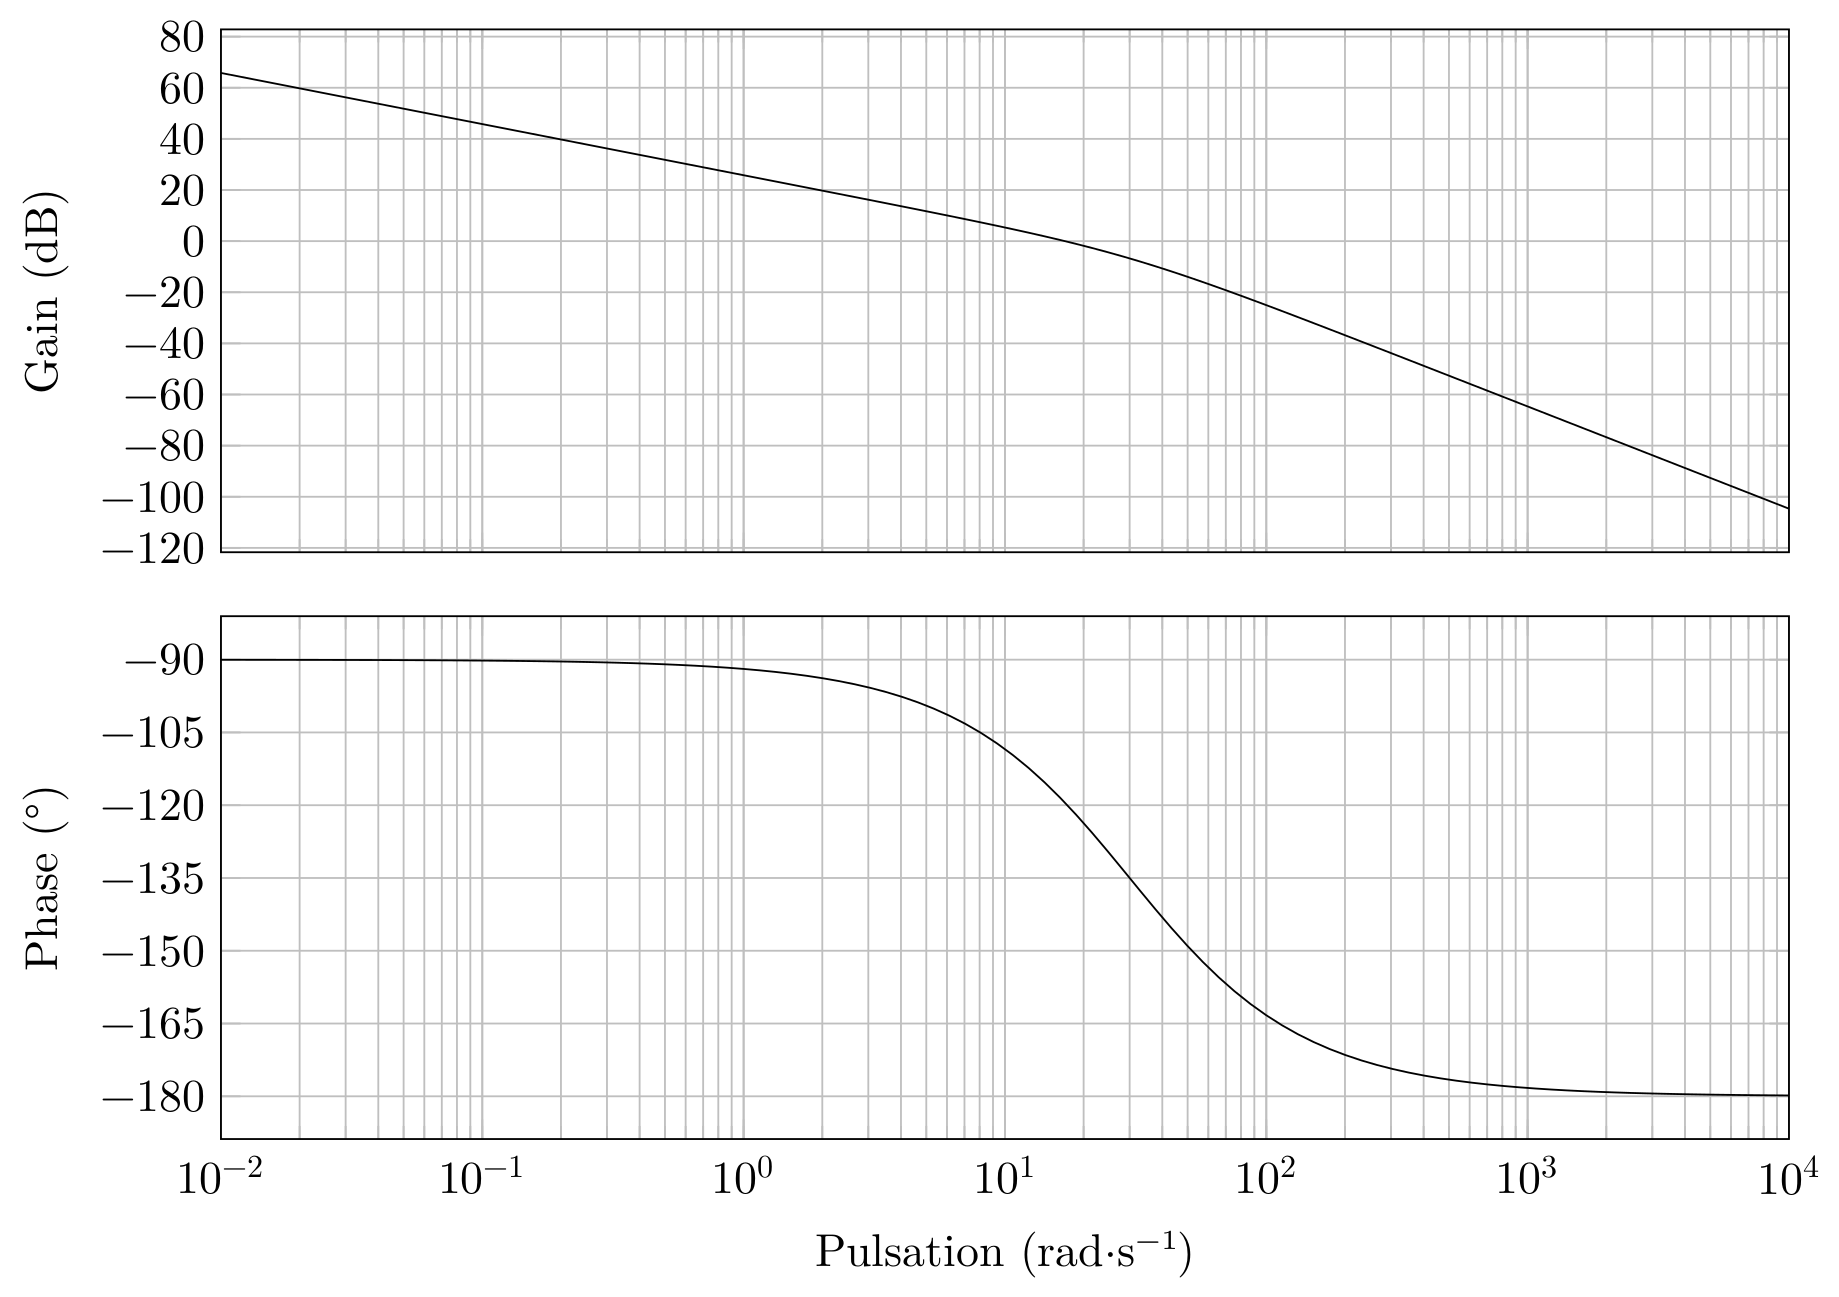
\includegraphics[width=0.9\linewidth]{img/figure_18}
 \caption{Diagramme de Bode en boucle ouverte avec $C(p)=1$}
 \label{img18}
\end{figure}
}{La phase part de -90\textdegree\ et va jusqu'à -180\textdegree, on en déduit qu'il s'agit d'un ordre 2, classe 1. Ce qui est confirmé par le diagramme de gain, pour lequel la pente commence à -20dB/decade et termine à -40dB/decade.

On a donc une FTBO de la forme $H(j\cdot\omega)=\frac{K}{j\cdot\omega\cdot (1+j\cdot\frac{\omega}{\omega_0})}$

La phase coupe -135\textdegree\ pour $\omega_0=30rad.s^{-1}$.

$H(j\cdot\omega_0)=\frac{K}{j\cdot\omega_0\cdot (1+j)}$

$G_{dB}(\omega_0)=20\cdot log\left(\frac{K}{\omega_0}\right)-20\cdot log(\sqrt{2})=20\cdot log\left(\frac{K}{\omega_0}\right)-3=-8$

Donc $20\cdot log\left(\frac{K}{\omega_0}\right)=-5$, donc $\frac{K}{\omega_0}=10^{\frac{-1}{4}}$

Donc $K=0.56\cdot \omega_0=16.8$
}

\end{document}